% This work is licensed under the Creative Commons
% Attribution-NonCommercial-ShareAlike 4.0 International License. To view a copy
% of this license, visit http://creativecommons.org/licenses/by-nc-sa/4.0/ or
% send a letter to Creative Commons, PO Box 1866, Mountain View, CA 94042, USA.

\addchap{Die Finite-Elemente-Methode}
\setcounter{section}{-1}
\section{Einleitung}
In diesem Dokument werden folgende Notationen verwendet:
\begin{itemize}
\item $u_x:=\frac{\partial u(x)}{\partial x}$ für die Ableitung einer diffbaren Funktion $u, x\mapsto u(x)$
\item $\frac{\partial u}{\partial n}:=\nabla u\cdot n$ wobei $n$ die Normale an $u$ ist
\end{itemize}

\subsection*{Durchbiegung einer Membran}
\begin{itemize}
\item Gegeben ist eine Membran als Graph der Funktion $u:\Omega\subseteq\R^2\to\R$.
\item Aus der Physik ist bekannt, dass die Deformationsarbeit proportional zur Flächenänderung ist. Die Flächenänderung ist
\begin{align*}
\frac{1}{2}\cdot\int\limits_\Omega\left(u^2_x+u_y^2\right)\d x\d y
\end{align*}
\item Die Energie des Systems ist 
\begin{align*}
\frac{1}{2}\cdot\int\limits_\Omega\left(u^2_x+u_y^2\right)\d x\d y-\int\limits_\Omega f\cdot u\d x\d y
\end{align*}
wobei $f$ eine von außen einwirkende Kraft ist
\item Es wirkt das \textbf{physikalische Minimierungsprinzip}, d.h. das System strebt stets einen Zustand minimaler Gesamtenergie an. Gesucht ist also eine Funktion $u$ derart, dass 
\begin{align*}
	E(u)&\leq E(v)&\forall v\in\tilde{V}\\
	\gdw ~ E(u)&\leq E(u+t\cdot v)\forall t\in\R,~&\forall v\in V
\end{align*}
Dabei ist $V$ ein Funktionenraum, dessen Funktionen auf dem Rand verschwinden.
\item Setze $\varphi(v,t):=E(u+t\cdot v)$, wobei $v$ als Parameter und $t$ als Variable aufgefasst wird. Somit lautet die notwendige Bedingung an das Energieminimum
\begin{align*}
\frac{\d\varphi}{\d t}(v,0)=0
\end{align*}
\end{itemize}
Nachrechnen:
\begin{align*}
\frac{\d\varphi}{\d t}(v,t)
&=\frac{\d}{\d t}E(u+t\cdot v)\\
&=\frac{\d}{\d t}\int\limits_\Omega\left(\frac{1}{2}\cdot\left((u+t\cdot v)_x^2+(u+t\cdot v)_y^2\right)-f(u+t\cdot v)\right)\d x\d y\\
&=\int\limits_\Omega\left((u+t\cdot v)_x\cdot v_x+(u+t\cdot v)_y\cdot v_y-f\cdot v\right)\d x\d y
\end{align*}
Setze nun $t:=0$. Dann folgt aus der notwendigen Bedingung
\begin{align*}
0=\int\limits_\Omega\left(u_x\cdot v_x+u_y\cdot v_y-f\cdot v\right)\d x\d y
\end{align*}
Es entsteht die Variationsaufgabe: Finde $u(t)$ so, dass 
\begin{align*}
\int\limits_\Omega u_x\cdot v_x+u_y\cdot v_y\d x\d y=\int\limits_\Omega f\cdot v\d x\d y~~~\forall v\in V.
\end{align*}

Durch partielle Integration (siehe Anhang für nähere Erklärung) erhält man aus dem linken Integral
\begin{align*}
\int\limits_\Omega u_x\cdot v_x+u_y\cdot v_y\d x\d y
=-\int\limits_\Omega\left(u_{xx}+u_{yy}\right)\cdot v
+\int\limits_{\partial\Omega}\underbrace{u_x\cdot v\cdot n_x+u_y\cdot v\cdot n_y}_{=(\nabla u\cdot n)\cdot v=0\text{, da $v=0$ auf }\partial\Omega}\d\gamma
\end{align*}
Somit folgt:
\begin{align*}
-\int\limits_\Omega\big(\underbrace{u_{xx}+u_{yy}}_{=\laplace u}\big)\cdot v\d x\d y=\int\limits_\Omega f\cdot v\d x\d y~\forall v\in V\\
\Longrightarrow-\laplace u\equiv f\text{ auf }\Omega\Longrightarrow\textbf{``Poisson-Gleichung''}
\end{align*}

\section{Sobolev-Räume}
Bezeichnungen für dieses Kapitel:

\begin{itemize}
\item $d\geq1$ sei die Raumdimension
\item $\Omega\subseteq\R^d$ sei offen und beschränkt
\item $p\in[1,\infty)$ reelle Zahl
\item $q\in(1,\infty]\mit\frac{1}{p}+\frac{1}{q}=1$ \textbf{konjungierter / dualer Exponent}
\item $\alpha=(\alpha_1,\ldots,\alpha_d)\in\N_0^d$ Multiindex mit
\begin{align*}
|\alpha|:=\alpha_1+\ldots+\alpha_d\\
D^\alpha\varphi:=\frac{\partial^{|\alpha|}\varphi}{\partial x_1^{\alpha_1}\hdots\partial x_d^{\alpha_d}}
\end{align*}
\item $L^p(\Omega):=\left\lbrace f:\Omega\to\R:f\text{ messbar und }\int\limits_\Omega |f(x)|^p\d\mathcal{L}(x)<\infty\right\rbrace$ Lebesgue-Räume
\end{itemize}

\textbf{Bemerkungen.}
\begin{enumerate}
\item Da $\Omega$ beschränkt ist, gilt $L^p(\Omega)\subseteq L^1(\Omega)$ und die kanonische Injektion ist stetig.
\item Es gilt die Gauß-Formel:
\begin{align}\label{GaussFormel}
\int\limits_\Omega\varphi\cdot D^\alpha\psi\d x=(-1)^{|\alpha|}\cdot\int\limits_\Omega\psi\cdot D^\alpha\varphi\d x~~~\forall \varphi,\psi\in C_0^\infty(\Omega)
\end{align}
\end{enumerate}

\begin{definition}[schwache Ableitung]
Seien $\varphi,\psi\in L^1(\Omega)$ und sei $\alpha\in\N_0^\alpha$ ein Multiindex. Dann heißt $\psi$ die \textbf{$\alpha$-te schwache Ableitung} von $\varphi:\gdw$
\begin{align*}
\forall v\in C_0^\infty(\Omega):\int\limits_\Omega\varphi\cdot D^\alpha v\d x=(-1)^{|\alpha|}\cdot\int\limits_\Omega\psi\cdot v\d x
\end{align*}
Kurzschreibweise: $\psi=D^\alpha\varphi$
\end{definition}

\textbf{Bemerkungen.}
\begin{enumerate}
\item Die $\alpha$-te schwache Ableitung ist eindeutig bestimmt im Sinne des $L^1$ (also bis auf Lebesgue-Nullmengen).
\item Ist $\varphi\in C^{|\alpha|}(\Omega)$, dann existiert die schwache $\alpha$-te 	Ableitung, die mit der klassischen Ableitung übereinstimmt.
\end{enumerate}

\begin{beisp}
$d=1$, $\Omega=(-1,1)$, $\varphi(x):=|x|$\\
Behauptung: $\varphi'(x)=\left\lbrace\begin{array}{cl}
-1, & \falls -1<x<0\\
1, & \falls 0\leq x<1
\end{array}\right.$\\
Die schwache Ableitung existiert also und der Wert an der Stelle 0 ist nicht relevant.
\begin{proof}
	Sei $v \in C_0^\infty(\Omega)$ beliebig. Dann
	\begin{align*}
		\int_{-1}^1 \varphi v' \d x &= \int_{-1}^0 \varphi v' \d x + \int_{0}^1 \varphi v' \d x \\
															&\stackeq{\text{part}} ~~~ \big[\varphi v\big]_{-1}^0 - \int_{-1}^0 (-1) v \d x + \big[\varphi v\big]_{0}^1 - \int_{0}^1 (1) v \d x \\
															&\stackeq{v = 0 \text{ auf Rand}} ~~~ - \int_{-1}^0 (-1) v \d x - \int_{0}^1 (1) v \d x \\
															&\stackeq{\text{Def}} - \int_{-1}^1 \varphi'(x)v\d x
	\end{align*}
\end{proof}
\end{beisp}

\begin{definition}[Sobolev-Räume]
Für $k\in\N_0$, $p\in[1,\infty)$ definieren wir den \textbf{Sobolev-Raum} wie folgt;
\begin{align}
W^{k,p}(\Omega):=\Big\lbrace\varphi\in L^p(\Omega):D^\alpha\varphi\text{ (schwache Abl.) existiert und }D^\alpha\varphi\in L^p(\Omega)~\forall|\alpha|\leq k\Big\rbrace
\end{align}
Als Norm vereinbaren wir
\begin{align*}
\Vert\varphi\Vert_{k,p,\Omega}:=\left(\sum\limits_{|\alpha|\leq k}\left\Vert D^\alpha\varphi\right\Vert^p_{L^p}\right)^{\frac{1}{p}}
=\left(\sum\limits_{|\alpha|\leq k}\int\limits_\Omega\left| D^\alpha\varphi(x)\right|^p\d x\right)^{\frac{1}{p}}
\end{align*}
Durch
\begin{align*}
|\varphi|_{k,p,\Omega}:=\left(\sum\limits_{|\alpha|= k}\left\Vert D^\alpha\varphi\right\Vert^p_{L^p}\right)^{\frac{1}{p}}
\end{align*}
wird eine Halbnorm definiert.\\
Für $p=2$ schreiben wir $H^k(\Omega):=W^{k,2}(\Omega)$.
\end{definition}

\begin{satz}[Eigenschaften der Sobolev-Räume]
Es gilt:
\begin{enumerate}
\item $\left(W^{k,p}(\Omega),\Vert\cdot\Vert_{k,p,\Omega}\right)$ ist ein Banachraum.
\item $C^\infty(\overline{\Omega})$ liegt dicht in $W^{k,p}(\Omega)$.
\item $H^k(\Omega)$ ist ein Hilbertraum mit dem Skalarprodukt
\begin{align*}
\langle \varphi,\psi\rangle_k:=\sum\limits_{|\alpha|\leq k}\int\limits_\Omega D^\alpha\varphi\cdot D^\alpha\psi\d x.
\end{align*}
\end{enumerate}
\end{satz}

\begin{satz}[Glätte von stückweise glatten Funktionen]\label{satz1.4}\enter
Seien $\Omega_1,\Omega_2\subseteq\Omega$ zwei nichtleere, offene, beschränkte und disjunkte Teilmengen mit stückweise glattem Rand. Gelte
$\overline{\Omega}=\overline{\Omega_1}\cup\overline{\Omega_2}$.
Weiterhin sei $\varphi\in L^p(\Omega)$ so, dass 
\begin{align*}
\exists k\geq 1:\forall i\in\lbrace1,2\rbrace:\varphi|_{\Omega_i}\in C^k(\overline{\Omega_i}).
\end{align*}
Dann gilt:
\begin{align*}
\varphi\in W^{k,p}(\Omega)\Longleftrightarrow\varphi\in C^{k-1}(\Omega)
\end{align*}
\end{satz}
\begin{proof}
Siehe Übung.
\end{proof}

\begin{definition}
Die Vervollständigung des $C_0^\infty(\Omega)$ bzgl. der Norm $\Vert\cdot\Vert_{k,p,\Omega}$ wird mit $W_0^{k,p}(\Omega)$ bezeichnet. Außerdem setze $H_0^k(\Omega):=W_0^{k,2}(\Omega)$.
\end{definition}

\begin{definition}[Lipschitz-Rand]\enter
$\Omega$ hat einen \textbf{Lipschitz-Rand} $:\gdw\exists N\in\N,\exists U_1,\ldots,U_N\subseteq\R^d$ offen, sodass
\begin{enumerate}
\item $
\begin{aligned}
\partial\Omega\subseteq\bigcup\limits^N_{i=1} U_i
\end{aligned}$
\item $
\begin{aligned}
\forall i\in\lbrace1,\ldots,N\rbrace:\partial\Omega\cap U_i
\end{aligned}$
 ist darstellbar als Graph einer Lipschitz-stetigen Funktion
\end{enumerate}
Das Gebiet $\Omega$ wird dann \textbf{Lipschitz-Gebiet} genannt.
\end{definition}

\begin{bemerkung}
Für Lipschitz-Gebiete existiert fast überall auf $\partial\Omega$ der äußere Normalenvektor.
\end{bemerkung}

\begin{satz}[Spursatz]\enter
Seien $\Omega$ eine Lipschitz-Gebiet, $k\in\N$, $l\in\lbrace 0,\ldots,k-1\rbrace$.\\
Dann gibt es eine stetige lineare Abbildung
\begin{align*}
\gamma_l:W^{k,p}(\Omega)\rightarrow L^p(\partial\Omega)
\end{align*}
mit der Eigenschaft
\begin{align*}
\gamma_l(\varphi)=\frac{\partial^l}{\partial u^l}\varphi|_{\partial\Omega}\qquad\forall\varphi\in C^k(\overline{\Omega}).
\end{align*}
\end{satz}

\begin{bemerkung}\
\begin{itemize}
\item $\gamma_0$ bildet die Funktion $\varphi$, die auf $\Omega$ lebt, auf ihre Randdaten ab.
\item  $\gamma_1$ gibt die Normalenableitung zurück.
\item Dass Bild von $W^{k,p}(\Omega)$ unter $\gamma_l$ ist ein abgeschlossener Unterraum von $L^p(\partial\Omega)$, genauer:
\begin{align*}
\gamma_l\left(W^{k,p}(\Omega)\right)=W^{k-l-\frac{1}{p},p}(\partial\Omega)
\end{align*}
\end{itemize}
\end{bemerkung}

\begin{satz}
Sei $\Omega$ ein Lipschitz-Gebiet. Dann gilt:
\begin{align*}
W_0^{k,p}(\Omega)=\left\lbrace\varphi\in W^{k,p}(\Omega):
\forall l\in\lbrace0,\ldots,k-1\rbrace:\gamma_l(\varphi)=0\right\rbrace
\end{align*}
\end{satz}

\begin{definition}
Seien $(X,\Vert\cdot\Vert_X)$ und $(Y,\Vert\cdot\Vert_Y)$ zwei normierte Vektorräume.
\begin{enumerate}
\item Eine lineare Abbildung $A:X\to Y$ heißt \textbf{kompakt} $:\gdw$ das Bild der abgeschlossenen Einheitskugel in $X$ im Raum $Y$ relativkompakt ist.
\item $X$ heißt \textbf{stetig eingebettet} in $Y$, in Zeichen $X\hookrightarrow Y:\gdw X\subseteq Y$ und die kanonische Injektion $I:X\to Y,~\varphi\mapsto\varphi$ stetig ist.
\item $X$ heißt \textbf{kompakt eingebettet} in $Y$, in Zeichen $X\stackrel{C}{\hookrightarrow} Y:\gdw X\subseteq Y$ und die kanonische Injektion $I:X\to Y,~\varphi\mapsto\varphi$ kompakt ist.
\end{enumerate}
\end{definition}

\begin{bemerkung}\
\begin{enumerate}
\item $X\hookrightarrow Y\Longrightarrow\exists c>0:\forall\varphi\in X:\Vert\varphi\Vert_Y\leq c\cdot\Vert\varphi\Vert_X$
\item $X\stackrel{C}{\hookrightarrow} Y\Longrightarrow X\hookrightarrow Y$
\item Ist $\stackrel{C}{\hookrightarrow} Y$ und $(\varphi_n)_{n\in\N}\subseteq X$ eine beschränkte Folge in $X$, so besitzt $(\varphi_n)_{n\in\N}\subseteq Y$ eine konvergente Teilfolge.
\end{enumerate}
\end{bemerkung}

\begin{satz}[Einbettung]\
\begin{enumerate}
\item Sei $p<d$. Dann gilt:
\begin{align*}
W^{k,p}(\Omega)\hookrightarrow W^{k-1,p}(\Omega)\qquad\forall q\in\left[1,\frac{p\cdot d}{d-p}\right]\\
W^{k,p}(\Omega)\stackrel{C}{\hookrightarrow} W^{k-1,p}(\Omega)\qquad\forall q\in\left[1,\frac{p\cdot d}{d-p}\right)
\end{align*}
\item Sei $p=d$. Dann gilt:
\begin{align*}
W^{k,p}(\Omega)\hookrightarrow W^{k-1,p}(\Omega)\qquad\forall q\in\left[1,\infty\right)
\end{align*}
\item Sei $k>\frac{d}{p}$. Dann gilt:
\begin{align*}
W^{k,p}(\Omega)\stackrel{C}{\hookrightarrow} C^l(\overline{\Omega})\qquad\forall 0\leq l\leq k-\frac{d}{p}
\end{align*}
\end{enumerate}
\end{satz}

\begin{bemerkung}\
\begin{itemize}
\item Es gilt stets
\begin{align*}
W^{k,p}(\Omega)\stackrel{C}{\hookrightarrow} W^{k-1,p}(\Omega)
\end{align*}
\item Falls $p=2$, $d\in\lbrace2,3\rbrace$: 
\begin{align*}
	H^2(\Omega)\hookrightarrow C(\overline{\Omega})
\end{align*}
Für $H^1(\Omega)$-Funktionen sind Punkte weiter nicht sinnvoll.
\item Falls $p=2,~d=2$: 
\begin{align*}
H^1(\Omega\stackrel{C}{\hookrightarrow} L^q(\Omega)\qquad\forall q\in[1,\infty)
\end{align*}
\item Falls $p=2,~d=3$: 
\begin{align*}
&H^1(\Omega)\stackrel{C}{\hookrightarrow} L^q(\Omega)\qquad\forall q\in[1,6)\\
&H^1(\Omega)\stackrel{C}{\hookrightarrow} L^6(\Omega)
\end{align*}
\end{itemize}
\end{bemerkung}

\begin{beisp}
	Für $d=2$ gibt es $H^1(\Omega)$-Funktionen, die nicht stetig sind:
	\begin{itemize}
		\item Sei $\Omega=$ Einheitskreis
		\item $u(x,y):=\ln\left(\ln\left(\frac{4}{\sqrt{x^2+y^2}}\right)\right)$
	\end{itemize}
	$u$ hat einen Pol im Ursprung, d.h. $u\not\in C(\overline{\Omega})$, aber:\enter
	\ul{Behauptung:} 
	\[\|u\|^2_{1,2,\Omega}\leq 8\pi + \frac{2\pi}{\ln(4)}< \infty\]
	\[\implies u \in H^1(\Omega)\]
	\begin{proof}
	\[\|u\|^2_{1,2,\Omega} = \underbrace{\int_\Omega |u|^2 \d x \d y}_{:=\text{ I}} +
	\underbrace{\int_\Omega |u_x|^2 + |u_y|^2 \d x \d y}_{:=\text{ II}}\]
	Es gilt für alle $z\geq 4$:
	\[\ln(\ln(z))\leq \sqrt{z}\]
	Mit der Koflächenformel erhalten wir:
	\begin{align*}
		\text{I} &= \int_\Omega |u|^2 \d x \d y \\
			&\leq \int_\Omega \left(\frac{4}{\sqrt{x^2 + y^2}}\right)^2 \d x \d y \\
			&\stackeq{\text{Koflä.}} \int_0^{2\pi}\int_0^1\left(\frac{4}{r}\right)^2 r \d r \d \varphi \\
			&= 8 \pi
	\end{align*}
	Als nächstes betrachten wir II. Dafür schauen wir uns zunächst die partiellen Ableitungen von $u$ an:
	\begin{align*}
		u_x &= \frac{1}{\ln\left(\frac{4}{r}\right)}\frac{r}{4}\left(-\frac{4}{r^2}\right)\frac{x}{r} = - \frac{x}{r^2\ln\left(\frac{4}{r}\right)} \\
		u_y &= - \frac{y}{r^2\ln\left(\frac{4}{r}\right)} \\
		\implies u_x^2 + u_y^2 &= \frac{x^2+y^2}{\left(r^2\ln\left(\frac{4}{r}\right)\right)^2} \\
		&= \frac{r^2}{\left(r^2\ln\left(\frac{4}{r}\right)\right)^2} \\
		&= \frac{1}{r^2\left(\ln\left(\frac{4}{r}\right)\right)^2} \\
	\end{align*}
	Also schlussendlich:
	\begin{align*}
		\text{II} ~~ &\stackeq{\text{vgl. I}} \int_0^{2\pi}\int_0^1\frac{r}{r^2\left(\ln\left(\frac{4}{r}\right)\right)^2} \d r \d \varphi \\
			 &= 2\pi \int_0^1 \frac{1}{r^2\left(\ln\left(\frac{4}{r}\right)\right)^2} \d r \\
			 &=\left[2\pi\left(\frac{1}{\ln\left(\frac{4}{r}\right)}\right)\right]_{r=0}^1 \\
			 &= \frac{2\pi}{\ln(4)}
	\end{align*}
\end{proof}
\end{beisp}

\newpage
\begin{proposition}\label{prop1.11}
Sei $\Omega\subseteq\R^d$ ein beschränktes Lipschitz-Gebiet und sei $F$ lineares, stetiges Funktional auf $H^1(\Omega)$ und $B$ eine beschränkte, symmetrische Bilinearform auf $H^1(\Omega)$ mit
\begin{align*}
B(u,u)\geq0\qquad\forall u\in H^1(\Omega).
\end{align*}
Sei $g$ eine Funktion mit $g(x)=1~\forall x\in\overline{\Omega}$ so, dass
\begin{align*}
|F(g)|+\sqrt{B(g,g)}>0.
\end{align*}
Dann gilt:\\
Die Normen $\Vert\cdot\Vert_{1,2,\Omega}$ und
\begin{align*}
\Vertiii{f}:=|f|_{1,2,\Omega}+|F(f)|+\sqrt{B(f,f)}
\end{align*}
sind äquivalent auf $H^1(\Omega)$, d. h. es existieren $c_1,c_2>0$ so, dass
\begin{align*}
c_1\cdot\Vert f\Vert_{1,2,\Omega}\leq\Vertiii{f}
\leq
c_2\cdot\Vert f\Vert_{1,2,\Omega}
\qquad\forall f\in H^1(\Omega)
\end{align*}
\end{proposition}
\begin{proof}\enter
	\underline{Zeige $\Vertiii{\cdot}$ ist eine Norm:}
Dies wird in der Übung gezeigt.\enter \enter
\underline{Zeige $\Vertiii{f}\leq c_2\cdot\Vert f\Vert_{1,2,\Omega}$:}
\begin{align*}
\Vertiii{f} &=
|f|_{1,2,\Omega}+|F(f)|+\sqrt{B(f,f)}\\
&\leq
\Vert f\Vert_{1,2,\Omega} +c_F\cdot\Vert f\Vert_{1,2,\Omega}+\sqrt{c_B\cdot\Vert f\Vert^2_{1,2,\Omega}}\\
&\leq
(1+c_F+\sqrt{c_B})\cdot\Vert f\Vert_{1,2,\Omega}
\end{align*}

%(iii)
\underline{Zeige $\Vert f\Vert_{0,2,\Omega}\leq c\cdot\Vertiii{f}$ indirekt:}
Angenommen es gibt eine Folge $(f_n)_{n\in\N}\subseteq H^1(\Omega)$ mit
\begin{align}\label{proof1.9}\tag{$\ast$}
\Vert f_n\Vert_{0,2,\Omega}=1\text{ und }\Vertiii{f_n}<\frac{1}{n}~\forall n\in\N
\end{align}
Dann gilt für alle $n\in\N$:
\begin{align*}
|f_n|_{1,2,\Omega}<\frac{1}{n}
\implies
\Vert f_n\Vert^2_{1,2,\Omega}\leq 2\
\end{align*}
Deshalb ist $(f_n)_{n\in\N}$ eine beschränkte Folge in $H^1(\Omega)$. Wegen $H^1(\Omega)\stackrel{C}{\hookrightarrow} L^2(\Omega)$ gibt eine Teilfolge $(f_m)_{m\in\N}$, die in $L^2(H)$ konvergiert.
\begin{align*}
&\stackrel{\eqref{proof1.9}}{\implies}
(f_m)_{m\in\N}\text{ ist eine Cauchy-Folge in }H^1(\Omega)\\
&\implies
 f_m\stackrel{m\to\infty}{\longrightarrow} f\in H^1(\Omega)\\
 &\implies
 \Vert f\Vert_{0,2,\Omega}=1\text{ und } |f|_{1,2,\Omega}=0\\
 &\implies
 f\text{ ist konstant, also } f\equiv \lambda\cdot g\mit\lambda\in\R
\end{align*}
Mit $\Vertiii{f}=0$ erhalten wir
\begin{align*}
\Vertiii{f} = 0 
&=|f|_{1,2,\Omega}+|F(f)|+\sqrt{B(f,f)}\\
&=0+|\lambda|\cdot|F(g)|+|\lambda|\cdot\sqrt{B(g,g)}\\
&=|\lambda|\cdot\underbrace{\Big(|F(g)|+\sqrt{B(g,g)}\Big)}_{>0}\\
&\implies\lambda=0\implies f\equiv 0
\end{align*}
Das ist ein Widerspruch zur Annahme $\Vert f\Vert_{0,2,\Omega}=1$. Also folgt
\begin{align*}
\Vert f\Vert_{0,2,\Omega}\leq c\cdot\Vertiii{f}\qquad\forall f\in H^1(\Omega).
\end{align*}

\underline{Zeige $\|f\|_{1,2,\Omega}\leq c_1 \Vertiii{f}$}

\begin{align*}
\Vert f\Vert_{1,2,\Omega}
&\leq
|f|_{1,2,\Omega}+\Vert f\Vert_{0,2,\Omega}\\
&\leq
\Vertiii{f}+c\cdot\Vertiii{f}\\
&=c_1\cdot\Vertiii{f}\qquad\forall f\in H^1(\Omega)
\end{align*}
\end{proof}

\begin{korollar}[Poincaré-Ungleichung]\enter %1.12
Aus Proposition \ref{prop1.11} folgt mit
\begin{align*}
B(u,v)=0\quad\text{ und }\quad F(u)=\int\limits_\Omega u(x)\d x
\qquad\forall u,v\in H^1(\Omega)
\end{align*}
die Äquivalenz der Normen
\begin{align*}
\Vert\cdot\Vert_{1,2,\Omega}\text{ und } |\cdot|_{1,2,\Omega}+|F(\cdot)|.
\end{align*}
Setze
\begin{align*}
V:=\left\lbrace\varphi\in H^1(\Omega):\int\limits_\Omega u(x)\d x=0\right\rbrace.
\end{align*}
Dann sind sogar $\Vert\cdot\Vert_{1,2,\Omega}$ und $|\cdot|_{1,2,\Omega}$ äquivalent auf $V$.
\end{korollar}
\begin{proof}
Es ist zu zeigen, dass $F$ ein lineares stetiges Funktional auf $H^1(\Omega)$  ist. Das ist einfach.
\end{proof}

\begin{proposition}[Friedrichs Ungleichung]\label{prop1.13FriedrichsUngleichung}\enter
$|\cdot|_{k,p,\Omega}$ ist eine Norm auf $W_0^{k,p}(\Omega)$, welche äquivalent zu der Norm $\Vert\cdot\Vert_{k,p,\Omega}$ ist.\\

Bemerkung: Für $k=1,~p=2$ ist das eine direkte Folgerung auf Proposition \ref{prop1.11} mit 
\begin{align*}
B(u,v)\equiv0\text{ und } F(u)=\int\limits_{\partial\Omega} u\d \gamma.
\end{align*}
\end{proposition}

\section{Abstrakte Variations-Analysis}
Die \textbf{Poissongleichung} ist
\begin{align}
	\left\{
	\begin{array}{r l l}\label{PoissonEquation}\tag{Poi}
		-\laplace u &\equiv f &\text{ auf }\Omega \\
		u &\equiv 0 &\text{ auf }\partial\Omega=:\Gamma.
	\end{array}\right.
\end{align}
Durch Multiplikation mit $v$ und Integration erhalten wir
\begin{align*}
&\stackrel{ v|_{\partial\Omega}\equiv0}{\implies}
\int\limits_\Omega f\cdot v\d x
=\int\limits_\Omega-\laplace u\cdot v\d x
=\int\limits_\Omega\nabla u\cdot\nabla v\d x-\underbrace{\int\limits_{\partial\Omega}\frac{\partial u}{\partial n}v\d x}_{=0}
\end{align*}
Definiere:
\begin{align*}
\text{Bilinearform } a(u,v)&:=\int\limits_\Omega\nabla u\cdot\nabla v\d x\\
\text{Linearform } l(v)&:=\int\limits_\Omega f\cdot v\d x
\end{align*}
$a$ und $l$ sind wohldefiniert für $f\in L^2(\Omega),~u,v\in H^1(\Omega)$. Um $v|_{\partial\Omega}=0$ und $u|_{\partial\Omega}=0$ sicherzustellen, muss $u,v\in H^1_0(\Omega)$ gelten.\\

\textbf{Variationsformulierung der Poissongleichung:}\\
Finde $u\in H_0^1(\Omega)$ so, dass
\begin{align*}
a(u,v)=l(v)\qquad\forall v\in H^1_0(\Omega).
\end{align*}
Dieses Problem gilt es zu lösen. Allgemeiner formuliert erhält man das folgende Problem:\\
Sei $V$ ein Hilbertraum. Finde $u\in V$ so, dass
\begin{align*}
a(u,v)=l(v)\qquad\forall v\in V.
\end{align*}

Eigenschaften der oben definieren Bilinearform $a$:
\begin{itemize}
\item $a$ ist stetig auf $V$, d. h.
\begin{align*}
\exists M>0:\forall u,v\in V:\big|a(u,v)\big|\leq M\cdot\Vert u\Vert_V\cdot\Vert v\Vert_V
\end{align*}
denn:
\begin{align*}
\big| a(u,v)\big|=\left|\int\limits_\Omega\nabla u\cdot\nabla v\d x\right|
\leq
|u|_{1,2,\Omega}\cdot|v|_{1,2,\Omega}
\leq
\underbrace{1}_{=:M}\cdot\Vert u\Vert_{1,2,\Omega}\cdot\Vert v\Vert_{1,2,\Omega}
\end{align*}
\item $a$ ist \textbf{koerziv}, d. h.
\begin{align*}
\exists\alpha>0:\forall v\in V:a(v,v)\geq\alpha\cdot\Vert v\Vert^2_V
\end{align*} 
denn:
\begin{align*}
a(v,v)
=\int\limits_\Omega\nabla v\cdot\nabla v\d x
=\int\limits_\Omega\sum\limits_{i=1}^d\left(\frac{\partial v}{\partial x_i}\right)^2\d x
=|v|^2_{1,2,\Omega}
\stackrel{\text{Fried}}{\geq}
\frac{1}{c_F^2}\cdot\Vert v\Vert^2_{1,2,\Omega}
\end{align*}
\end{itemize}
Eigenschaften der oben definierten Linearform $l$:
\begin{itemize}
\item $l$ ist stetig auf $V$, d. h.
\begin{align*}
\exists M^\ast>0:\forall v\in V: \big|l(v)\big|\leq M^\ast\cdot\Vert v\Vert_V
\end{align*}
denn:
\begin{align*}
\big| l(v)\big|=\left|\int\limits_\Omega f\cdot v\d x\right|
\stackrel{\text{CS}}{\leq}
\Vert f\Vert_{0,2,\Omega}\cdot\Vert v\Vert_{0,2,\Omega}
\stackrel{\text{CS}}{\leq}
\underbrace{\Vert f\Vert_{0,2,\Omega}}_{=:M^\ast}\cdot\Vert v\Vert_{1,2,\Omega}
\end{align*}
\end{itemize}

\begin{theorem}[Lax-Milgram]\label{theorem2.1LaxMilgram}\enter
Sei $V$ ein Hilbertraum, $a$ eine stetige, koerzive Bilinearform auf $V$ und $b$ eine stetige Linearform auf $V$.\\
Dann hat das Variationsproblem
\begin{align*}
\text{Bestimme $u\in V$ so, dass }a(u,v)=b(v)\qquad\forall v\in V.
\end{align*}
eine eindeutige Lösung.
\end{theorem}
\begin{proof}
\underline{Schritt 1:}\\ Transformation in einen dualen Operator über dem Dualraum $V^\ast$ von $V$. Die Abbildung $v\mapsto a(u,v)$ definiert für alle festen $u\in V$ eine stetige Linearform auf $V$. Wir bezeichnen diese mit $Au\in V^\ast$
\begin{align*}
	\langle Au,v\rangle=(Au)(v):&=a(u,v)\qquad\forall u,v\in V \\
	b\in V^\ast: \langle b,v\rangle&=b(v)
\end{align*}
Damit folgt:
\begin{align*}
\text{Variationsproblem}&\Longleftrightarrow\langle Au,v\rangle=\langle b,v\rangle\qquad\forall v\in V\\
&\Longleftrightarrow Au=b\text{ in }V^\ast
\end{align*}
\underline{Schritt 2:}\\
Die Abbildung $V\to V^\ast$ kann auch als Abbildung $A:V\to V$ aufgefasst werden. Eigenschaften von $A$:
\begin{enumerate}[label=(\alph*)]
\item $A$ ist linear auf $V$
\begin{align*}
\big\langle A(\alpha u+\beta v),w\big\rangle
&=a(\alpha u+\beta v,w)\\
&=\alpha a(u,w)+\beta a(v,w)\\
&=\alpha\langle Au,w\rangle+\beta\langle Av,w\rangle\qquad\forall u,v,w,\in V
\end{align*}
\item $A$ ist stetig auf $V$:
\begin{align*}
\Vert A v\Vert_{V}
&=\Vert A u\Vert_{V^\ast}\\
&=\sup\limits_{v\neq0}\frac{\big|\langle Au,v\rangle\big|}{\Vert v\Vert_V}\\
&=\sup\limits_{v\neq0}\frac{\big|a(u,v)\big|}{\Vert v\Vert_V}\\
&\leq
\sup\limits_{v\neq0}\frac{M\cdot\Vert u\Vert_V\cdot\Vert v\Vert_V}{\Vert v\Vert_V}\\
&=M\cdot\Vert u\Vert_V
\end{align*}
\end{enumerate}
\underline{Schritt 3:} Setze
\begin{align*}
u^{n+1}:=P(u^n):=u^n+\tau\cdot(b-A u^n)\qquad\forall\tau\in\R_{\neq0}
\end{align*}
$u^0$ ist eine beliebiger Startwert.
\begin{align*}
P:V\to V,\qquad u\mapsto u+\tau\cdot(b-Au)
\end{align*}
Jeder Fixpunkt von $P$ ist eine Lösung von $Au=b$ und umgekehrt.\\
Es bleibt also zu zeigen, das $P$ einen eindeutigen Fixpunkt hat. Dafür nutzen wir den \textit{Banach'schen Fixpunktsatz} \ref{BanachscherFixpunktsatz}.\\

Wähle also $N=V$. $P$ ist eine Kontraktion, wenn $\tau$ richtig gewählt wird.
\begin{align*}
&\quad\Vert P(u)-P)v)\Vert^2_V\\
&=\big\langle P(u)-P(v),P(u)-P(v)\big\rangle_V\\
&=\big\langle u-v-\tau\cdot A(u-v),u-v-\tau\cdot A(u-v)\big\rangle_V\\
&=\langle u-v,u-v\rangle_V-2\cdot\tau\cdot\underbrace{\big\langle A(u-v),u-v\big\rangle_V}_{\stackrel{\text{Def.}}{=}a(u-v,u-v)\stackrel{\text{koerz}}{\geq}\alpha\cdot\Vert u-v\Vert^2_V}+\tau^2\cdot\underbrace{\big\langle A(u-v),A(u-v)\big\rangle_V}_{=\Vert A(u-v)\Vert^2_V\leq M^2\cdot\Vert u-v\Vert^2_V}\\
&\stackrel{\tau>0}{\leq}
\Vert u-v\Vert^2_V\cdot\big(1-2\cdot\tau\cdot\alpha+\tau^2\cdot M^2\big)
\end{align*}
Wähle $\tau:=\frac{\alpha}{M^2}>0$. Dann gilt:
\begin{align*}
1-2\cdot\tau\cdot\alpha+\tau^2\cdot M^2=1-\frac{\alpha^2}{M^2}>0
\end{align*}
$P$ ist eine Kontraktion, also hat $P$ nach dem Banachschen Fixpunktsatz einen eindeutigen Fixpunkt und damit hat auch $Au=b$ eine eindeutige Lösung.
\end{proof}

Schwierigkeit:
\begin{align*}
a(u,v)=b(v)\qquad\forall v\in V
\end{align*}
ist ein unendlichdimensionales Problem.\\
\underline{Idee:} Approximation in einem endlich-dimensionalen Unterraum\\
Sei $V_h\subseteq V$ ein endlich-dimensionaler Unterraum von $V$. Betrachte das Problem
\begin{align*}
\text{Finde }u_n\in V_h \text{ so, dass }\qquad \\
a(u_n,v_h)=l(v_h)\qquad\forall v_h\in V_h
\end{align*}
Da $a$ und $l$ auf $V_h$ die Voraussetzungen des Satzes von Lax-Milgram auf $V_h$ erfüllen, gibt es ein eindeutiges $u_n\in V_h$, das das Problem löst.\\

Sei $\lbrace\varphi_i\rbrace_{i=1}^n$ eine Basis von $V_h$.
\begin{align*}
\Big(a(u_n,v_h)=l(v_h)\qquad\forall v_h\in V_h\Big)\Longleftrightarrow
\Big(a(u_n,\varphi_i)=l(\varphi_i)\qquad\forall i\in\lbrace1,\ldots,n\rbrace\Big)
\end{align*}
und 
\begin{align*}
u_n=\sum\limits_{j=1}^n u_j\cdot\varphi_j,\qquad u_1,\ldots,u_n\in\R,j\\
\sum\limits_{j=1}^n a(\varphi_j,\varphi_i)\cdot u_j=l(\varphi_i)\qquad\forall i\in\lbrace1,\ldots,n\rbrace\\
\end{align*}
Daraus ergibt sich ein lineares Gleichungssystem:
\begin{align*}
\left.\begin{array}{ll}
A:=(a_{i,j})_{i,j=1,\ldots,n} &a_{i,j}:=a\big(\varphi_j,\varphi_i\big)\\
b:=(b_i)_{i=1,\ldots,n} &b_i:=l(\varphi_i)\\
u:=(u_j)_{j=1,\ldots,n}
\end{array}\right\rbrace A\cdot u=b\qquad\text{ LGS}
\end{align*}

\begin{theorem}[Céa's Lemma]\enter
Sei $V$ ein Hilbertraum, $V_h\subseteq V$ ein abgeschlossener Unterraum, $a$ eine stetige, koerzive Bilinearform auf $V$ und $l$ eine stetige Linearform. Dann gilt:
\begin{align*}
\exists C=\frac{M}{\alpha}>0:\Vert u-u_n\Vert_V\leq C\cdot\inf\limits_{v_h\in V_h}\Vert u-v_h\Vert_V
\end{align*}
\end{theorem}
\begin{proof}
\begin{align*}
a(u,v)&=l(v) &\forall v\in V\\
a(u_n,v_h)&= l(v_h) &\forall v_h\in V_h\subseteq V
\end{align*}
Wir erhalten die sogenannte \textbf{Galerkin Orthogonalität}, indem wir die Differenz dieser beiden Gleichungen bilden: (nutze $v=v_h$ in der ersten Gleichung!) 
\begin{align}\label{eqGalerkinOrthogonalitaet}\tag{GalerkinOrtho}
a(u-u_n,v_h)=0\qquad v_h\in V_h
\end{align}
Also:
\begin{align*}
\alpha\cdot\Vert u-u_n\Vert^2_V
&\leq
a(u-u_n,u-u_n)\\
&=a(u-u_n,u-v_v+v_h- u_n)\\
&=a(u-u_n,u-v_h)+\underbrace{a(u-u_n,\underbrace{v_h-u_n}_{\in V_h})}_{=0}\\
&\stackrel{\text{stetig}}{\leq}
M\cdot\Vert u-u_n\Vert_V\cdot\Vert u-v_h\Vert_V\\
\implies
\Vert u-u_n\Vert_V&\leq\frac{M}{\alpha}\cdot\Vert u-v_h\Vert_V\qquad\forall v_h\in V_h\\
\implies
\Vert u-u_n\Vert_V&\leq \frac{M}{\alpha}\cdot\inf\limits_{v_h\in V_h}\Vert u-v_h\Vert_V
\end{align*}
\end{proof}

\begin{theorem}[Dualitätsargument, Aubin-Nietsche]\enter
Sei $V$ ein Hilbertraum, $V_h\subseteq V$ ein abgeschlossener Unterraum, $a$ eine stetige, koerzive Bilinearform und $l$ eine stetige Linearform. Sei weiterhin $H$ ein Hilbertraum mit Skalarprodukt $\langle\cdot,\cdot\rangle_H$ und Norm $\Vert\cdot\Vert_H$ so, dass $V\hookrightarrow H$ und $V$ liegt dicht in $H$ bzgl. $\Vert\cdot\Vert_H$. Sei zusätzlich $u_\varphi\in V$ für jedes feste $\varphi\in H$ die eindeutige Lösung von
\begin{align}\label{Dtheorem2.3}\tag{D}
a(v,u_\varphi)=\langle\varphi,v\rangle_H\qquad\forall v\in V
\end{align}
Dann gilt:
\begin{align*}
\Vert u-u_h\Vert_H\leq M\cdot\Vert u-u_h\Vert_V\cdot\sup\limits_{\begin{subarray}{c}\varphi\in H\\\Vert\varphi\Vert_H=1\end{subarray}}\inf\limits_{v_h\in V}\Vert u_\varphi-v_h\Vert_V
\end{align*}
\end{theorem}

\begin{proof}
$v\mapsto\langle\varphi,v\rangle_H$ ist eine stetige Linearform auf $V$. Aus Lax-Milgram \ref{theorem2.1LaxMilgram} folgt, dass es eine eindeutige Lösung $u_\varphi\in V$ gibt.
 
\begin{align*}
\langle u-u_h,\varphi\rangle_H
&=\langle\varphi,u-u_h\rangle_H\\
&=a(u-u_h,u_\varphi)\\
&=a(u-u_h,u_\varphi-v_h)\mit v_h\in V\text{ beliebig}\\
&\leq M\cdot\Vert u-u_h\Vert_V\cdot\Vert u_\varphi-v_h\Vert_V\\
\Vert u-u_h\Vert_H
&=\sup\limits_{\begin{subarray}{c}\varphi\in H\\\Vert\varphi\Vert=1\end{subarray}}\langle u-u_h,\varphi\rangle_H\\
&\leq M\cdot\Vert u-u_h\Vert_V\cdot\sup\limits_{\begin{subarray}{c}\varphi\in H\\\Vert\varphi\Vert=1\end{subarray}}\inf\limits_{v_h\in V}\Vert u_\varphi-v_h\Vert_V
\end{align*}
\end{proof}

\begin{theorem}\label{theorem2.4} %2.4
Seien $(X,\Vert\cdot\Vert_X)$, $(Y,\Vert\cdot\Vert_Y)$ Banachräume  mit $X\stackrel{C}{\hookrightarrow} Y$ und $a_0,a_1$ stetige Bilinearformen auf $X$. Gelte weiterhin:
\begin{itemize}
\item $a_0$ ist symmetrisch und koerziv auf $X$
\item $\begin{aligned}
\exists A>0:\forall u,v\in X:\big|a_1(u,v)\big|\leq A\cdot\Vert u\Vert_X\cdot\Vert v\Vert_Y
\end{aligned}$
\end{itemize}
Erfülle
\begin{align*}
a(u,v):=a_0(u,v)+a_1(u,v)\qquad\forall u,v\in X
\end{align*}
die Ungleichung
\begin{align*}
a(v,v)>0\qquad\forall v\in X\setminus\lbrace0\rbrace.
\end{align*}
Dann sind die beiden Probleme
\begin{align*}
\text{Finde }u\in X\text{ so, dass }
a(u,v)=l(v)\qquad\forall v\in X\\
\text{Finde }\tilde{u}\in X\text{ so, dass }
a(v,\tilde{u})=l(v)\qquad\forall v\in X
\end{align*}
jeweils eindeutig lösbar für alle stetigen Linearformen $l$.
\end{theorem}

\begin{theorem} %2.5
Gleiche Voraussetzungen wie Theorem \ref{theorem2.4}.\\
Sei zusätzlich $X_h\subseteq X$ ein endlich-dimensionaler Unterraum von $X$.\\
Dann ist das Problem
\begin{align*}
\text{Finde }u_h\in X_h\text{ so, dass }
a(u_h,v_h)=l(v_h)\qquad\forall v_h\in X_h
\end{align*}
eindeutig lösbar für jede feste stetige Linearform $l$. Zusätzlich gilt
\begin{align*}
\Vert u-u_h\Vert_X\leq\frac{M}{\alpha}\cdot\inf\limits_{v_h\in X_h}\Vert u-u_h\Vert_X
\end{align*}
unter der Voraussetzung
\begin{align*}
a(v,v)&\geq\beta\cdot\Vert v\Vert^2_X &\forall v\in X\\
\big|a(u,v)\big|&\leq M\cdot\Vert u\Vert_X\cdot\Vert v\Vert_Y &\forall u,v\in X
\end{align*}
\end{theorem}

\section{Schwache Lösungen} %3.
Hier: skalare, lineare, elliptische partielle Differentialgleichungen zweiter Ordnung, also
\begin{align*}
-\sum\limits_{i,j=1}^d\frac{\partial}{\partial x_i}\left(A_{i,j}(x)\cdot\frac{\partial u}{\partial x_j}\right)+\sum\limits_{i=1}^d a_i(x)\cdot\frac{\partial u}{\partial x_i}+\alpha(x)\cdot u=f(x)\text{ in }\Omega
\end{align*}
Vereinfachende Annahmen:
\begin{align*}
\begin{array}{ll}
	f\in L^2(\Omega)&\alpha \in C(\Omega)\\
	a_i\in C^1(\Omega),i\in\lbrace1,\ldots,d\rbrace, & A_{i,j}\in C^1(\Omega), i,j\in\lbrace1,\ldots,d\rbrace\\
	A_{i,j}(x)=A_{j,i}(x)\forall x\in\Omega, i,j\in\lbrace1,\ldots,d\rbrace, & a=\big(a_1,\ldots a_d\big)^T\\
	A=\big(A_{i,j}\big)^d_{i,j=1},& 0<\lambda_0:=\inf\limits_{x\in\Omega}\inf\limits_{z\in\R^d\setminus\lbrace0\rbrace}\frac{z^T\cdot A(x)\cdot z}{z^T\cdot z}
\end{array}
\end{align*}

\subsection*{Einige Spezialfälle}
\begin{itemize}
\item Poisson-Gleichung: $\alpha\equiv 0,~a\equiv0,~A=I$
\item Membran-Gleichung: $\alpha\equiv0,~a\equiv 0$
\item Reaktionsdiffusionsgleichung: $a\equiv 0$
\item Konvektions-Diffusions-Gleichung: ist der allgemeine Fall
\end{itemize}

\subsection*{Randbedingungen}
\begin{itemize}
\item Die \textbf{homogene Dirichlet-Randbedingung} ist
\begin{align*}
u\equiv0\qquad\text{auf}\qquad\Gamma:=\partial\Omega
\end{align*}
\item Die \textbf{Neumann-Randbedingung} ist
\begin{align*}
n^T\cdot A\cdot\nabla u\equiv q\qquad\text{auf}\qquad\Gamma,\qquad\forall g\in L^2(\Gamma)
\end{align*}
wobei $n$ der äußere Normalenvektor ist.
\item Mischform: Dirichlet-Randbegingung auf $\Gamma_D$ und Neumann-Randbedingung auf $\Gamma_N$ für $\Gamma=\Gamma_D\stackrel{\cdot}{\cup}\Gamma_N,~\Gamma_D\cap\Gamma_N=\emptyset$
\item Die \textbf{Robin-Randbedingung} ist
\begin{align*}
\gamma\cdot u+n^T\cdot A\cdot\nabla u\equiv h\qquad\text{auf}\qquad\Gamma
\end{align*}
\end{itemize}

%Was ist das hier?
Nun bringen wir die allgemeine Form der Gleichung von oben in eine lesbare Form.
Sei dazu $v\in C_0^\infty(\Omega)$. Wir multiplizieren auf beiden Seiten mit v und integrieren anschließend über ganz $\Omega$. Dann gilt:
\begin{align*}
\int\limits_\Omega f\cdot v\d x
&\stackeq{\text{Def}}
\int\limits_\Omega-\sum\limits_{i,j=1}^d\frac{\partial}{\partial x_i}\left(A_{i,j}(x)\cdot\frac{\partial u}{\partial x_j}\right)\cdot v+\sum\limits_{i=1}^d a_i(x)\cdot\frac{\partial u}{\partial x_i}\cdot v+\alpha(x)\cdot u\cdot v\d x\\ 
&\stackeq{\text{partGauß}}
\int\limits_\Omega\sum\limits_{i,j=1}^d A_{i,j}(x)\cdot\frac{\partial u}{\partial x_j}\cdot\frac{\partial v}{\partial x_i}\d x+\int\limits_\Omega\sum\limits_{i=1}^d a_i(x)\cdot\frac{\partial u}{\partial x_i}\cdot v+\alpha(x)\cdot u\cdot v\d x\\
&\qquad
-\underbrace{\int\limits_\Gamma\underbrace{\sum\limits_{i,j=1}^d n_i\cdot A_{i,j}(x)\cdot\frac{\partial u}{\partial x_j}}_{=n^T\cdot A\cdot\nabla u}\cdot v\d\gamma}_{=0}\\
&=
\int\limits_\Omega\nabla u^T\cdot A\cdot\nabla v+a\cdot\nabla u\cdot v+\alpha\cdot u\cdot v\d x
\end{align*}

\begin{definition}[Schwache Lösung]\ %3.1
\begin{enumerate}[label=(\roman*)]
\item Eine Funktion $u\in H_0^1(\Omega)$ heißt \textbf{schwache Lösung einer Konvektions-Diffusions-Gleichung mit homogener Dirichlet-Randbedingung}
\begin{align*}
:\Longleftrightarrow
\int\limits_\Omega\nabla u^T\cdot A\cdot\nabla v+a\cdot\nabla u\cdot v+\alpha\cdot u\cdot v\d x
=\int\limits_\Omega f(x)\cdot v\d x
\qquad\forall v\in H_0^1(\Omega)
\end{align*}
\item Eine Funktion 
\begin{align*}
u\in H_D^1(\Omega):=\big\lbrace\varphi\in H^1(\Omega):\varphi|_{\Gamma_D}\equiv 0\big\rbrace
\end{align*}
heißt \textbf{schwache Lösung einer Konvektions-Diffusions-Gleichung  mit gemischten Randbedingungen}
\begin{align*}
:\Longleftrightarrow
\int\limits_\Omega \nabla u^T\cdot A\cdot\nabla v+a\cdot\nabla u\cdot v+\alpha\cdot u\cdot v\d x
=\int\limits_\Omega f(x)\cdot v\d x+\int\limits_{\Gamma_N}g\cdot v\d\gamma
\qquad\forall v\in H^1_D(\Omega)
\end{align*}
\item Eine Funktion $u\in H^1(\Omega)$ heißt \textbf{schwache Lösung einer Konvektions-Diffusions-Gleichung mit Neumann-Randbedingung}
\begin{align*}
:\Longleftrightarrow
\int\limits_\Omega\nabla u^T\cdot A\cdot\nabla v+a\cdot\nabla u\cdot v+\alpha\cdot u\cdot v\d x
=\int\limits_\Omega f(x)\cdot v\d x+\int\limits_{\Gamma} g\cdot v\d\gamma
\qquad\forall v\in H^1(\Omega)
\end{align*}
\end{enumerate}
\end{definition}

\begin{bemerkung}\ %NoNumber
\begin{itemize}
\item Jede ``klassische'' Lösung ist auch eine schwache Lösung. 
\item Jede schwache Lösung, welche glatt genug ist ($C^2$) ist auch eine ``klassische'' Lösung.
\item schwächere Annahmen an die Problemdaten:
\begin{align*}
	&\alpha\in L^\infty(\Omega), &&\alpha\geq0\\
	&a_i\in L^\infty(\Omega), &&\div(a)=\sum\limits_{i=1}^d\frac{\partial a_i}{\partial x_i}\in L^\infty(\Omega)\\
&A_{i,j}\in L^\infty(\Omega)
\end{align*}
\item Unter der inhomogenen Dirichletbedingung
\begin{align*}
u|_\Gamma\equiv u_D
\end{align*}
gehört die schwache Lösung zu
\begin{align*}
u_D+H_0^1(\Omega)=\big\lbrace v\in H^1(\Omega):v|_\Gamma\equiv u_D\big\rbrace
\end{align*}
Der Testraum ist immer $H^1_0(\Omega)$.
\end{itemize}
\end{bemerkung}

\begin{theorem}[Existenz und Eindeutigkeit von schwachen Lösungen]\ 
\begin{enumerate}[label=(\roman*)]
\item Sei 
\begin{align*}
\alpha-\frac{1}{2}\cdot\div(a)\geq0.
\end{align*}
Dann hat die Konvektions-Diffusions-Gleichung mit homogenen Dirichlet-Randbedingungen eine eindeutige schwache Lösung.
\item Sei 
\begin{align*}
\alpha-\frac{1}{2}\cdot\div(a)\geq0\qquad\text{ und }\qquad a\cdot n\geq0\text{ auf }\Gamma_N.
\end{align*}
Dann hat die Konvektions-Diffusions-Gleichung mit gemischten Randbedingungen eine eindeutige Lösung.
\item Sei 
\begin{align*}
\alpha-\frac{1}{2}\cdot\div(a)\geq0,\qquad \alpha\geq\alpha_0>0\qquad\text{ und }\qquad a\cdot n\geq 0\text{ auf }\Gamma.
\end{align*}
Dann hat die Konvektions-Diffusions-Gleichung mit Neumann-Randbedingung eine eindeutige Lösung.
\item Sei
\begin{align*}
\alpha=0,\qquad-\frac{1}{2}\cdot\div(a)=0\qquad\text{und}\qquad a\cdot n\geq 0\text{ auf }\Gamma\\
\end{align*}
und gelte
\begin{align*}
	\int\limits_\Omega f(x)\d x+\int\limits_\Gamma g\d\gamma=0.
\end{align*}
Dann hat die Konvektions-Diffusions-Gleichung mit Neumann-Randbedingung eine eindeutige schwache Lösung $u$, welche 
\begin{align*}
\int\limits_\Omega u(x)\d x=0
\end{align*}
erfüllt.
\end{enumerate}
\end{theorem}

\begin{proof}
\underline{Zeige (i):}\\
$V=H_0^1(\Omega)$, $\Vert\cdot\Vert_V=\Vert\cdot\Vert_{1,2,\Omega}\sim\vert\cdot\vert_{1,2,\Omega}$. 
Zeige zunächst, dass $l(v)$ stetig ist. %Zuerst die rechte Seite: <- steht bei mir ursprünglich auch so im Skript, aber ich versteh es nicht. Macht wenig Sinn an der Stelle.
\begin{align*}
l(v)&=\int\limits_\Omega f\cdot v\d x\\
|l(v)|&\leq\Vert f\Vert_{0,2}\cdot\Vert v\Vert_{0,2}\\
			&\leq\Vert f\Vert_{0,2}\cdot\Vert v\Vert_{1,2}
\end{align*}
Bilinearform
\begin{align*}
a(v,w)=\int\limits_\Omega\nabla v^T\cdot A\cdot\nabla w+\big(a\cdot\nabla v+\alpha\cdot v\big)\cdot w\d x
\end{align*}
Stetigkeit:
\begin{align*}
\big|a(v,w)\big|&=\left|\int\limits_\Omega\nabla v^T\cdot A\cdot\nabla w+\big(a\cdot\nabla v+\alpha\cdot v\big)\cdot w\d x\right|\\
&\leq
\Vert A\Vert_{L^\infty}\cdot\Vert\nabla v\Vert_{0,2}\cdot\Vert\nabla w\Vert_{0,2}\\
&\quad+\Vert a\Vert_{L^\infty} \cdot\Vert\nabla v\Vert_{0}\cdot\Vert w\Vert_{0,2}\\
&\quad+\Vert\alpha\Vert_{L^\infty}\cdot\Vert v\Vert_{0,2}\cdot\Vert w\Vert_{0,2}\\
&\leq
\left(\Vert A\Vert_{L^\infty}+\Vert a\Vert_{L^\infty}+\Vert\alpha\Vert_{L^\infty}\right)\cdot\Vert v\Vert_{1,2}\cdot\Vert w\Vert_{1,2}
\end{align*}
Koerzivität: 
\begin{align*}
a(v,v)&\geq\underbrace{\beta}_{>0}\cdot\Vert v\Vert^2_{1,2}\qquad\forall v\in V=H_0^1(\Omega)\\
a(v,v)&=
\int\limits_\Omega\nabla v^T\cdot A\cdot\nabla v+\big(a\cdot\nabla v+\alpha\cdot v\big)\cdot v\d x\\
&=\int\limits_\Omega\nabla v^T\cdot A\cdot\nabla v+\big(a\cdot\nabla v\big) v+\alpha\cdot v^2\d x\\
&=\int\limits_\Omega\nabla v^T\cdot A\cdot\nabla v+\frac{a}{2}\nabla \left(v^2\right)+\alpha\cdot v^2\d x\\
&=\int\limits_\Omega\underbrace{\nabla v^T\cdot A\cdot\nabla v}_{\geq\lambda_0\cdot|\nabla v(x)|^2\geq0}+\underbrace{\left(\alpha-\frac{1}{2}\cdot\div(a)\right)}_{\stackrel{\text{Vor}}{\geq}0}\cdot v^2\d x+\underbrace{\int\limits_{\Gamma}\frac{1}{2}\cdot(a\cdot n)\cdot v^2\d\gamma}_{=0}\\
&\geq
\lambda_0\cdot |v|^2_{1,2}\\
&\stackrel{\text{Fried}}{\geq}
\frac{\lambda_0}{C_f^2}\cdot\Vert v\Vert^2_{1,2}
\end{align*}

\underline{Zeige (ii):}\\
Homogene Dirichlet-Randbedingungen auf $\Gamma_D$ und Neumann-Randbedingungen auf $\Gamma_N$.
\begin{align*}
	\left\{\begin{array}{rl}
			\alpha-\frac{1}{2}\cdot\div(a)\geq0 &\text{ in }\Omega\\
			a\cdot n\geq0&\text{ auf }\Gamma_N
\end{array}\right.
\end{align*}
Also gilt
\begin{align*}
l(v)&=\int\limits_\Omega f\cdot v\d x+\int\limits_{\Gamma_N}g\cdot v\d\gamma\\
\big|l(v)\big|&\leq\underbrace{\Vert f\Vert_{0,2}}_{\leq\Vert v\Vert_{1,2}}\cdot\Vert v\Vert_{0,2}+\Vert g\Vert_{0,2,\Gamma}\cdot\underbrace{\Vert v\Vert_{0,2,\Gamma_N}}_{\leq\Vert v\Vert_{1,2,\Omega}}
\end{align*}
Erinnerung:
\begin{align*}
H^1_D(\Omega)=\big\lbrace v\in H^1(\Omega):v|_{\Gamma_D}\equiv 0\big\rbrace
\end{align*}
Die Abschätzung für $a$ ist analog zu (a), nur ist das letzte Integral nicht Null, sondern:
\begin{align*}
\int\limits_\Gamma\frac{1}{2}\cdot(a\cdot n)\cdot v^2\d\gamma
&=\underbrace{\int\limits_{\Gamma_D}\frac{1}{2}\cdot(a\cdot n)\cdot v^2\d\gamma}_{=0}+\underbrace{\int\limits_{\Gamma_N}\frac{1}{2}\cdot\underbrace{(a\cdot n)}_{\geq0}\cdot v^2\d\gamma}_{\geq0}
\end{align*}

\underline{Zeige (iii):}
\begin{align*}
	\left\{\begin{array}{rl}
\alpha-\frac{1}{2}\cdot\div(a)\geq0&\text{ in }\Omega\\
\alpha\geq\alpha_0>0&\text{ in }\Omega\\
a\cdot n\geq0&\text{ auf }\Gamma
	\end{array}\right.
\end{align*}
Wende Theorem \ref{theorem2.4} an:
\begin{align*}
X&=H^1(\Omega),\qquad Y=L^2(\Omega)\\
l(v)&=\int\limits_\Omega f\cdot v\d x+\int\limits_\Gamma g\cdot v\d\gamma\\
a_0(v,w)&=\int\limits_\Omega\nabla v^T\cdot A\cdot\nabla w+\alpha\cdot v\cdot w\d x\\
a_1(v,w)&=\int\limits_\Omega(a\cdot\nabla v)\cdot v\d x
\end{align*}
Stetigkeit von $l$ und $a_0$ sowie Symmetrie sind klar. Bleibt nur Koerzivität zu zeigen:
\begin{align*}
a(v,v)&=\int\limits_\Omega\nabla v^T \cdot A \cdot \nabla v+\underbrace{\alpha}_{\geq\alpha_0>0}\cdot v^2\d x\\
&\geq\lambda_0\cdot|v|^2_{1,2,\Omega}+\alpha_0\cdot\Vert v\Vert^2_{0,2,\Omega}\\
&\geq\underbrace{\min\lbrace\lambda_0,\alpha_0\rbrace}_{>0}\cdot\Vert v\Vert^2_{1,2,\Omega}
\end{align*}
Stetigkeit von $a_1$:
\begin{align*}
\big| a_1(v,w)\big|&\leq\Vert a\Vert_{L^\infty}\cdot\underbrace{|\nabla v|_{0,2,\Omega}}_{\leq\Vert v\Vert_{1,2,\Omega}}\cdot\underbrace{\Vert w\Vert_{0,2,\Omega}}_{\leq\Vert w\Vert_{1,2,\Omega}}
\end{align*}
Es bleibt nur noch zu zeigen, dass
\begin{align*}
a(v,v)>0\qquad\forall v\in H^1(\Omega)\setminus\lbrace0\rbrace
\end{align*}
Also
\begin{align*}
a(v,v)
&=\int\limits_{\Omega} \nabla v^T\cdot A\cdot \nabla v+\underbrace{(a\cdot\nabla v)\cdot v}_{=\frac{a}{2}\cdot\nabla(v^2)}+\alpha\cdot v^2\d x\\
&=\int\limits_{\Omega}\nabla v^T\cdot A\cdot\nabla v+\underbrace{\left(\alpha-\frac{1}{2}\cdot\div(a\right)}_{\geq0}\cdot v^2\d x+\int\limits_\Gamma\frac{1}{2}\cdot\underbrace{(a\cdot n)}_{\geq0}\cdot v^2\d\gamma\\
&\geq\lambda_0\cdot |v|^2_{1,2,\Omega}\\
&\geq 0\qquad\forall v\in H^1(\Omega)
\end{align*}
Aber wir müssen noch den Fall \dq$=0$\dq{} ausschließen. Also ist zu zeigen, dass
\begin{align*}
a(v,v)=0\implies v\equiv 0
\end{align*}
gilt.
\begin{align*}
0&=a(v,v)\geq\underbrace{\lambda_0}_{>0}\cdot|v|^2_{1,2,\Omega}\geq0 \\
\implies& |v|_{1,2,\Omega}=0 \\
\implies& v\equiv c\text{ konstant auf }\Omega\\
0&=a(c,c)=\int\limits_\Omega\underbrace{\nabla c^T}_{=0}\cdot A\cdot\underbrace{\nabla c}_{=0}+(a\cdot\underbrace{\nabla c}_{=0})\cdot c+\alpha\cdot c^2\d x\\
&=\int\limits_\Omega\alpha\cdot c^2\d x\\
&\geq\underbrace{\alpha_0}_{>0}\cdot\Vert c\Vert^2_{0,2,\Omega}\\
&\implies\Vert c\Vert_{0,2,\Omega}=0\\
&\implies c=0\\
&\implies v\equiv 0
\end{align*}

\underline{Zeige (iv):}
\begin{align*}
	\left\{\begin{array}{rl}
a\cdot n=0&\text{ auf }\Gamma\\
\alpha=0,~\div(a)=0&\text{ in  }\Omega\\
\end{array}\right. 
\end{align*}
\begin{align*}
	V=\left\lbrace v\in H^1(\Omega):\int\limits_\Omega v(x)\d x=0\right\rbrace\mit|\cdot|_{1,2}\sim\Vert\cdot\Vert_{1,2}\text{ (siehe Poincaré-Ungleichung)}
\end{align*}
Also sind die Bilinearform
\begin{align*}
a(v,w)=\int\limits_\Omega\nabla v^T\cdot A\cdot\nabla w+(a\cdot\nabla v)\d x
\end{align*}
und die Linearform 
\begin{align*}
l(v)=\int\limits_\Omega f(x)\cdot v(x)\d x+\int\limits_\Gamma g\cdot v\d\gamma
\end{align*}
stetig. Zur Koerzivität:
\begin{align*}
a(v,v)&=\int\limits_\Omega\nabla v^T\cdot A\cdot\nabla v+(a\cdot\nabla v)\cdot v\d x\\
&=\int\limits_\Omega\nabla v^T\cdot A\cdot \nabla v-\Big(\frac{1}{2}\cdot\underbrace{\div(a)}_{=0}\Big)\cdot v^2\d x+\int\limits_\Gamma\frac{1}{2}\cdot\underbrace{(a\cdot n)}_{=0}\cdot v^2\d\gamma\\
&\geq\lambda_0\cdot|v|_{1,2,\Omega}^2\\
&\geq\frac{\lambda_0}{C^2_p}\cdot\Vert v\Vert^2_{1,2,\Omega}
\end{align*}
Aus Lax Milgram \ref{theorem2.1LaxMilgram} folgt, dass das Variationsproblem eine eindeutig Lösung \ul{in $V$} hat. Aber: Die schwache Lösung benötigt $X=H^1(\Omega)$. Wir wissen, dass das Problem
\begin{align*}
\text{Finde $u\in V$ so, dass }a(u,v)=l(v)\qquad\forall v\in V
\end{align*}
eine eindeutige Lösung besitzt. Es bleibt zu zeigen, dass $a(u,\indi)=l(\indi)$ für eine konstante Funktion $\indi$ gilt.
\begin{align*}
a(u,\indi)=l(\indi)
&\Longleftrightarrow
\int\limits_\Omega\underbrace{\nabla u^T\cdot A\cdot\nabla\indi}_{=0}+(a\cdot\nabla u)\cdot\indi\d x
=
\int\limits_\Omega f(x)\d x+\int\limits_\Gamma g\d\gamma\stackeq{\text{Vor}}0\\
&\Longleftrightarrow
a\cdot \nabla u=0\\
&\stackrel{\text{part. Int.}}{\Longleftrightarrow}
0=-\int\limits_\Omega\underbrace{(\div(a))}_{\equiv0}\cdot u\d x+\int\limits_\Gamma\underbrace{(a\cdot n)}_{\equiv 0}\cdot u\d\gamma
\end{align*}
Also ist die schwache Lösung in $V$ die schwache Lösung in $H^1$, die wir gesucht haben.
\end{proof}

\begin{theorem}[Regularität]\label{theorem3.3}\enter
	Sei $\Gamma$ eine $C^1$-Mannigfaltigkeit oder $\Omega$ konvex und $f\in L^2(\Omega)$. Wenn wir Neumann-Randbedingungen betrachten und wir annehmen, dass es eine Funktion 
\begin{align*}
u_g\in H^2(\Omega)\mit g=\tilde{\gamma}_{1,N}(u_g)
\end{align*}
gibt. Dann gilt:
\begin{align*}
\Vert u\Vert_{2,2,\Omega}\leq C\cdot\Big(\Vert f\Vert_{0,2,\Omega}+\Vert u\Vert_{2,2}\Big)
\end{align*}
wobei $C$ nur von $\Omega, A,a,\alpha$ abhängt (also nicht von $f$).
\end{theorem}

\section{Finite-Elemente Räume} %4
\begin{definition}[1D finite Elemente]\enter
Sei $\Omega=(0,1)\subseteq\R$. Sei
\begin{align*}
\mathcal{T}_n:=\big\lbrace I_j:0\leq j\leq n\big\rbrace\mit I_j:=\big(t_j,t_{j+1}\big)
\end{align*}
und 
\begin{align*}
0=t_0<t_1<\ldots<t_n< t_{n+1}=1
\end{align*}
eine Zerlegung von $(0,1)$. Weiterhin setze
\begin{align*}
h_j:=t_{j+1}-t_j,\qquad h:=\max\limits_{0\leq j\leq n} h_j
\end{align*}
Für $k\in\N_0$ und $m\in\N_0$ definiere
\begin{align*}
S_h^{k,-1}&:=\Big\lbrace\varphi:[0,1]\to\R:\varphi\big|_{I_j}\in P_k,~0\leq j\leq n\Big\rbrace\\
S_h^{k,m}&:=S_n^{k,-1}\cap C^m\big([0,1]\big)\\
S_{h,0}^{k,m}&:=\Big\lbrace\varphi\in S_n^{k,m}:\varphi(0)=\varphi(1)=0\Big\rbrace
\end{align*}
Hierbei ist $P_k$ der Raum der Polynome von höchstens Grad $k$.\\ Die Funktionen in $S_h^{k,m}$ heißen \textbf{finite-Elemente-Funktionen}.

\begin{figure}[h!]
	\begin{center}
	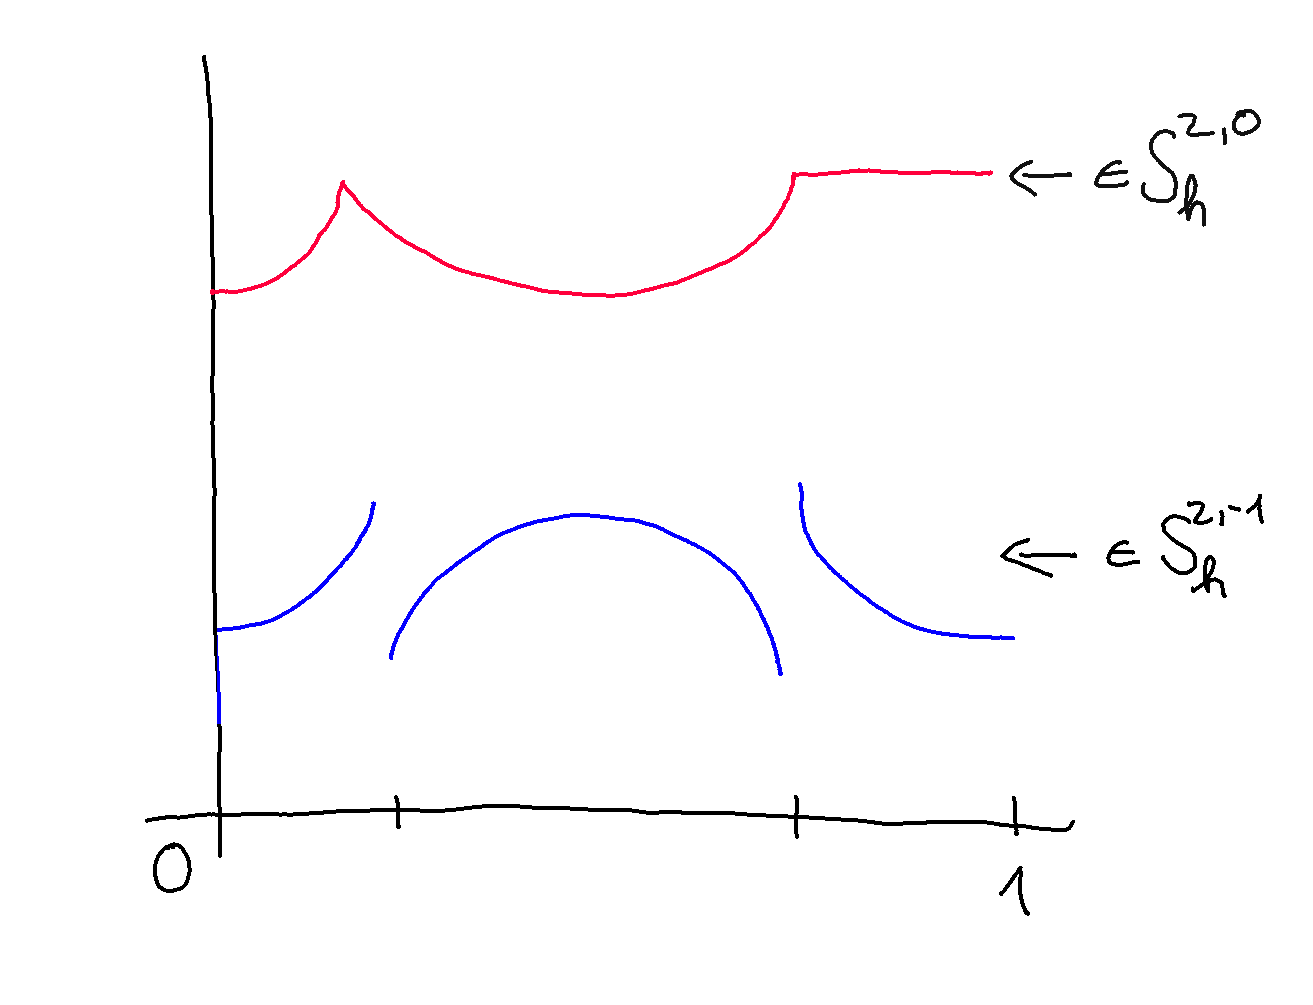
\includegraphics[width=0.75\textwidth]{pics/Sketch0.png}
	\caption{Beispiel für finite-Elemente-Funktionen}
	\label{AbbFiniteFunktionen}
	\end{center}
\end{figure}
\end{definition}

\begin{bemerkung}\
\begin{itemize}
\item Für $m=k-1$ erhält man Splines.
\item $\begin{aligned}
S_h^{k,m}\subseteq H^{m+1}(\Omega)
\end{aligned}$ wegen Satz \ref{satz1.4}
\item $\begin{aligned}
S_h^{0,m}
\end{aligned}$ sind konstante Funktionen auf $(0,1)$ für $m\geq0$
\item Die Räume haben folgende Dimensionen:
\begin{align*}
\dim\left(S_h^{k,-1}\right)&=(n+1)\cdot(k+1)\\
\dim\left(S_h^{k,m}\right)&=\dim\left(S_h^{k,-1}\right)-n\cdot(m+1)\\
\dim\left(S_{h,0}^{k,m}\right)&=\dim\left(S_h^{k,m}\right)-2\\
\end{align*}
Konkrete wichtige Beispiele:
\begin{align*}
\dim\left(S_h^{k,0}\right)&=(n+1)\cdot(k+1)-n\\
\dim\left(S_{h,0}^{k,0}\right)&=(n+1)\cdot(k+1)-n-2=(n+1)\cdot(k-1)+n\\
\dim\left(S_{h,0}^{1,0}\right)&=(n+1)\cdot 2-n-2=n\\
\dim\left(S_{h,0}^{2,0}\right)&=(n+1)\cdot 3-n-2=2\cdot n+1\\
\end{align*}
\end{itemize}
\end{bemerkung}
%RobertToDo: Polishing of the following
Sei $\lbrace\varphi_j\rbrace_{j\in J}$ eine Basis von $S_h^{k,0}$
%=\langle\lbrace\varphi_j\rbrace\rangle$
und Lösung $u_h\in S_{h,0}^{k,0}: u_h=\sum\limits_j u_j\cdot\varphi_j$\\
Diskretes Problem: Finde $u_h\in S_{h,0}^{k,0}$ so, dass 

\begin{align*}
	&a(u_h,\varphi_h)=l(\varphi_h)&\qquad&\forall \varphi_h\in S_{h,0}^{k,0}\\
	\Longleftrightarrow &a(u_h,\varphi_i)=l(\varphi_i)&\qquad&\forall i
\end{align*}
In Matrix-Notation ergibt dies Folgendes:
\begin{align*}
	&A=(a_{i,j}),&&a_{i,j}:=a(\varphi_j,\varphi_i)\\
	&b=(b_i),&&b_i:=l(\varphi_i)
\end{align*}
\begin{align*}
\Longleftrightarrow A\cdot U=b,\qquad U=(u_i)
\end{align*}
Hierbei heißt $A$ \textbf{Stiffness-Matrix}.

\begin{align*}
	&S^{1,0}_{h,0}=\text{span}\big\lbrace\varphi_i:1\leq i\leq n\big\rbrace,\qquad
\varphi_i(t)=\left\lbrace\begin{array}{cl}
\frac{t-t_{i-1}}{h_{i-1}}, &\falls t\in I_{i-1}\\
\frac{t_{i+1}-t}{h_i}, &\falls t\in I_i\\
0, &\sonst
\end{array}\right.\\
\big(&\text{supp}(\varphi_i) = [t_{i-1}, t_{i+1}]\big)
\end{align*}
\begin{align*}
\implies a_{i,j}=0\text{ für }|i-j|>1\implies A\text{ ist Tridiagonalmatrix}
\end{align*}

\begin{figure}[h!]
	\begin{center}
		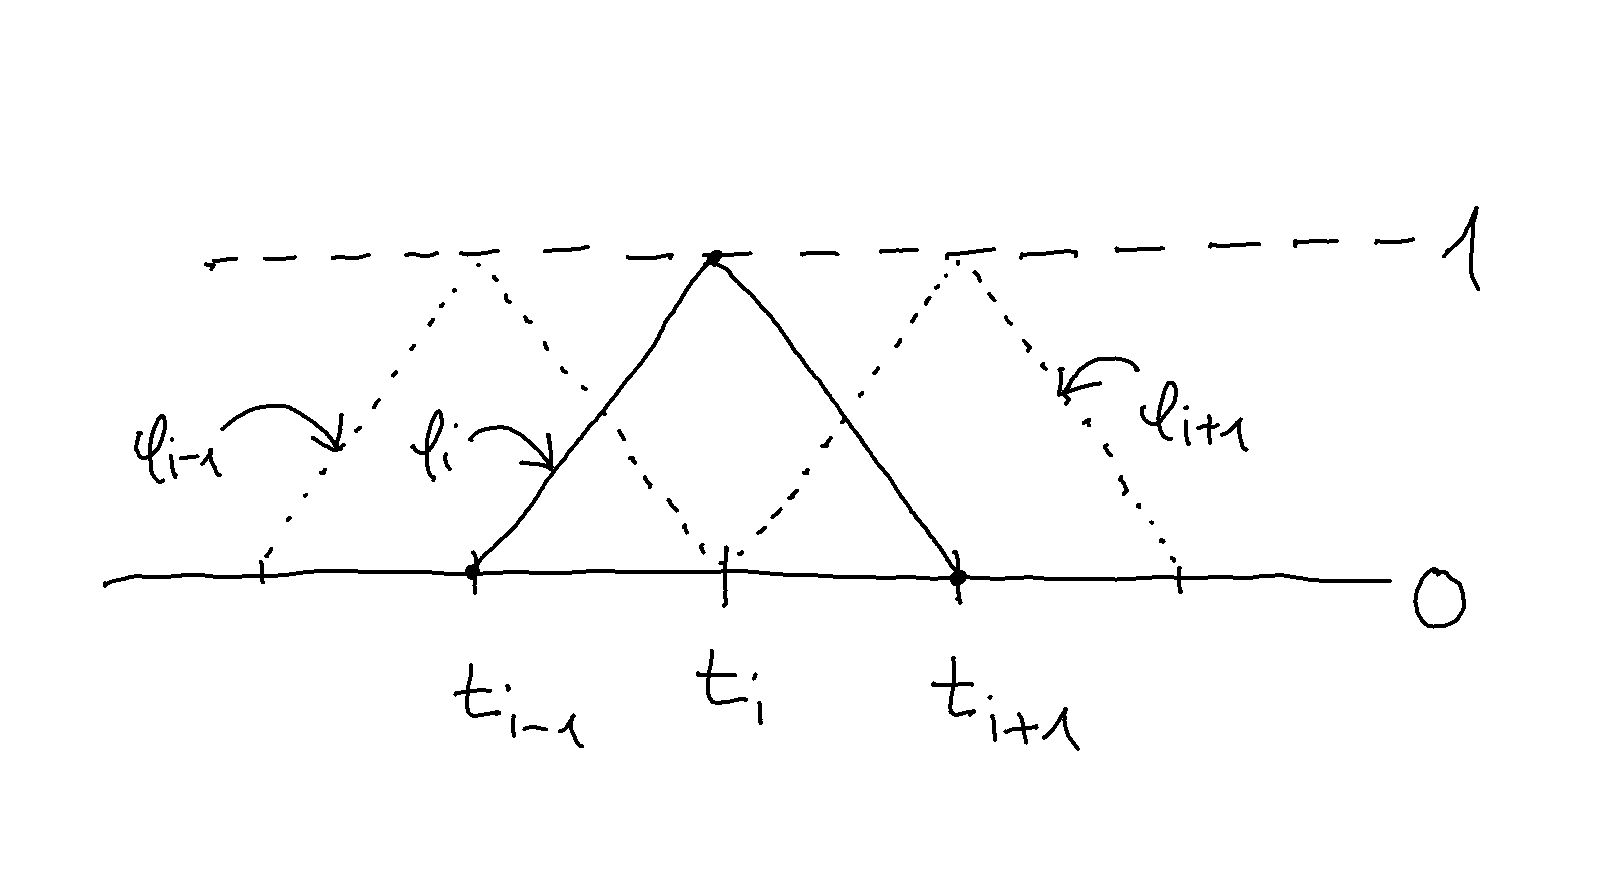
\includegraphics[width=0.75\textwidth]{pics/Sketch1.png}
		\caption{Hut-Funktionen}
		\label{AbbHutFunktionen}
	\end{center}
\end{figure}

\begin{figure}[h!]
\begin{center}
%\begin{figure}[!h]
	\centering
	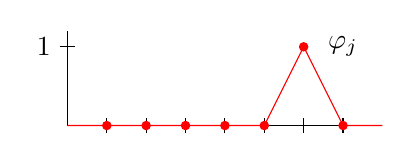
\begin{tikzpicture}[scale=1]

	
	%\fill[black!20!white] (2.15,0) -- ++(0,0.35) -- ++(0.65,0.26) -- ++(0,-0.61) -- cycle;
	%\draw (2.15,0) 
	\draw (0,0) -- ++(0,1.2);
	\draw (0,0) -- ++(4,0);

	% Funktion
	\draw[red] (0,0) -- ++(2.5,0) -- ++(0.5,1) -- ++(0.5,-1) -- ++(0.5,0);
	
	% Anstrich Y-Achse 
	\draw (-0.1,1) -- ++(0.2,0);
	
	% Anstriche X-Achse
	\draw (0.5,-0.1) -- ++(0,0.2);
	\draw (1  ,-0.1) -- ++(0,0.2);
	\draw (1.5,-0.1) -- ++(0,0.2);
	\draw (2  ,-0.1) -- ++(0,0.2);
	\draw (2.5,-0.1) -- ++(0,0.2);
	\draw (3  ,-0.1) -- ++(0,0.2);
	\draw (3.5,-0.1) -- ++(0,0.2);
	
	
	\filldraw[red] (0.5,0) circle (1.5pt);
	\filldraw[red] (1  ,0) circle (1.5pt);
	\filldraw[red] (1.5,0) circle (1.5pt);
	\filldraw[red] (2  ,0) circle (1.5pt);
	\filldraw[red] (2.5,0) circle (1.5pt);
	\filldraw[red] (3  ,1) circle (1.5pt);
	\filldraw[red] (3.5,0) circle (1.5pt);
	
	
	\node at (-0.3,1) {1};
	\node at (3.5,1) {$\varphi_j$};
	%\node at (2.8,-0.1) {b};
	%\node at (2.15,0.53) {f(a)};
	%\node at (2.77,0.71) {f(b)};
	
	\end{tikzpicture}
%\end{figure}
\caption{einzelne Hut-Funktione}
\label{AbbPhiHat}
\end{center}
\end{figure}

\begin{align*}
S_{h,0}^{2,0}&=\spann\big\lbrace\varphi_1,\ldots,\varphi_n,\psi_0,\ldots,\psi_n\big\rbrace,\qquad
\psi_i(t)=\left\lbrace\begin{array}{cl}
4\cdot\frac{(t-t_i)\cdot(t_{i+1}-t)}{h_i^2}, &\falls t\in I_i\\
0 &\sonst
\end{array}\right.
\end{align*}

\begin{figure}[h!]
	\begin{center}
		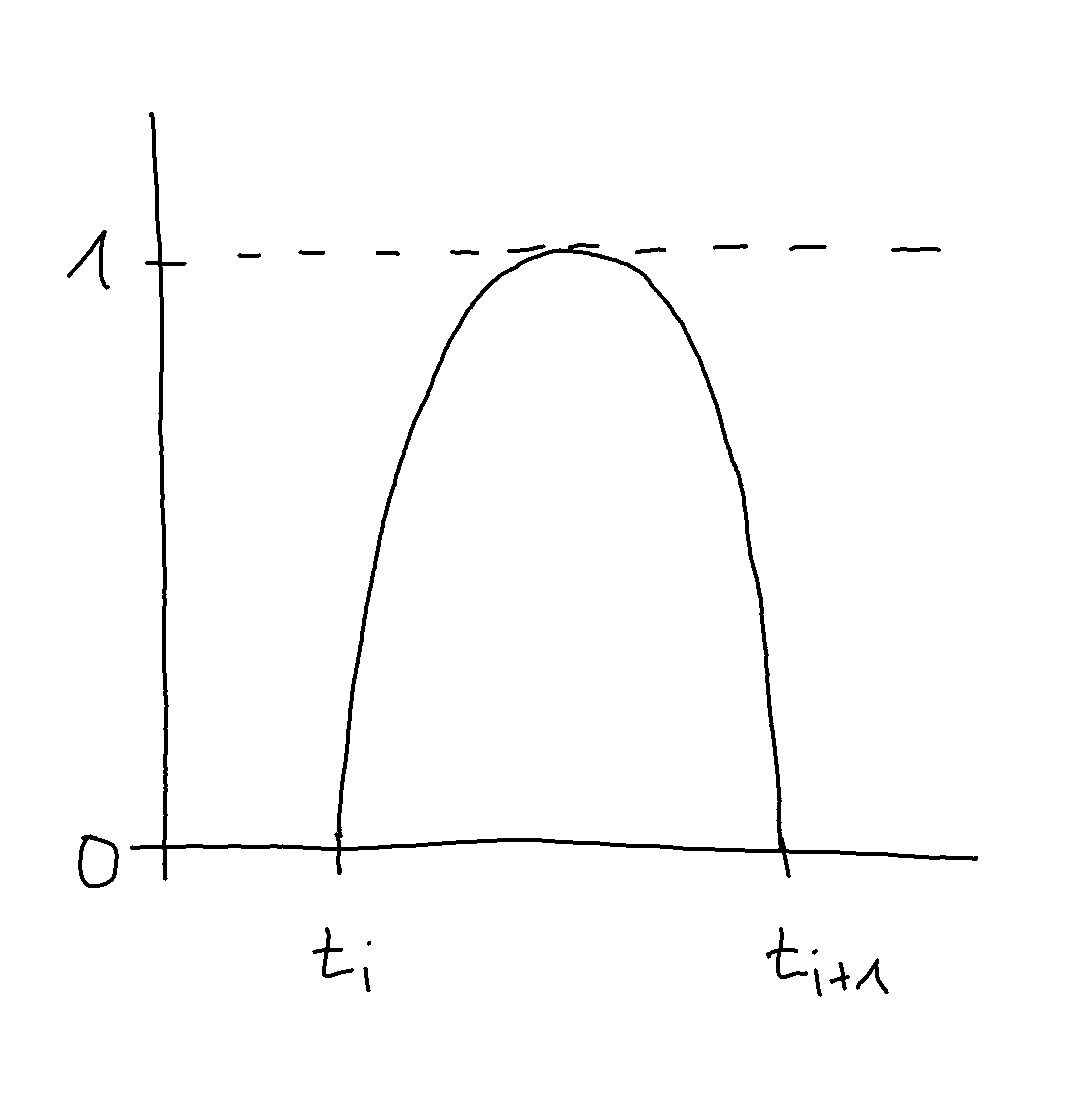
\includegraphics[width=0.5\textwidth]{./pics/Sketch2.png}
		\caption{einzelne zweifach diffbare finite-Elemente-Funktion}
		\label{AbbFiniteElementeFunktionZweifachDiffbar}
	\end{center}
\end{figure}

Die Stiffness-Matrix $A$ lässt sich als Blockmatrix schreiben:
\begin{align*}
A=\begin{pmatrix}
A_{LL} & A_{LQ}\\
A_{QL} & A_{QQ}
\end{pmatrix}
\end{align*}
wobei $A_{QQ}$ eine Diagonalmatrix ist. Somit:
\begin{align*}
\begin{pmatrix}
A_{LL} & A_{LQ}\\
A_{QL} & A_{QQ}
\end{pmatrix}\cdot\begin{pmatrix}
U_L\\ U_Q
\end{pmatrix}=
\begin{pmatrix}
b_L\\ b_Q
\end{pmatrix}
\end{align*}
Dieses System von Gleichungen ist äquivalent zu:
\begin{align*}
\big(A_{LL}-A_{LQ}\cdot A^{-1}_{QQ}\cdot A_{QL}\big)\cdot U_L&= b_L-A_{LQ}\cdot A^{-1}_{QQ}\cdot b_Q\\
A_{QQ}\cdot U_Q&= b_Q-A_{QL}\cdot U_L
\end{align*}

\begin{theorem}[Approximationseigenschaft von 1D finiten Elementen]\label{theorem4.2}\enter
Sei $u\in H^{k+1}(\Omega)\cap H^{1}_0(\Omega)$ für ein $k\geq1$. Dann gilt:
\begin{align*}
	\inf\limits_{v_h\in S_{h,0}^{k,0}}\big|u-v_h\big|_{1,2}\leq h^k\cdot|u|_{k+1,2}
\end{align*}
(Hierbei ist $h$ wie oben der Maximalabstand.)
\end{theorem}
\begin{proof}
Definiere Intervallweise die Funktion auf $I_i$ durch
\begin{align*}
v_h^\ast(t):=L_i(t)\qquad\forall t\in I_i,~\forall i\in\lbrace1,\ldots,n\rbrace
\end{align*}
wobei die $L_i$ die Lagrange-Interpolationen in $P_k$ bzgl. $t_i+\frac{s}{h}\cdot h_i,~0\leq j\leq h$ sind.\\
Offenbar gilt $v_h^\ast\in S^{k,0}_{h,0}$. \\
$u-v_n^\ast$ in $\overline{I_i}=[t_i,t_{i+1}]$ hat $(k+1)$ Nullen wegen der Interpolation. Somit hat $\big(u-v_h^\ast)^{(\mu)}$ $(k+1-\mu)$ Nullen.
\begin{align*}
\big|u-v_h^\ast\big|_{\mu,2,I_i}
&=\left\Vert \big(u-v_h^\ast\big)^{(\mu)}\right\Vert_{0,2,I_i}\\
&\stackrel{\ref{TODO}}{\leq}
h_i\cdot\left|\big(u-v_h^\ast\big)^{(\mu)}\right|_{1,2,I_i}\\
&=h_i\cdot\left|\big(u-v_h^\ast\big)^{(\mu+1)}\right|_{0,2,I_i}\\
&\leq h_i\cdot\left|u-v_h^\ast\right|_{\mu+1,2,I_i}\\
\end{align*}
\begin{align*}
\implies
\big|u-v_h^\ast\big|_{1,2,I_i}
&\leq h_i^k\cdot\big|u-v_h^\ast\big|_{k+1,2,I_i} \\
&\stackeq{v_h^\ast|_{I_i}\in P_k}h_i^k\cdot |u|_{k+1,2,I_i}
\end{align*} 
Somit folgt
\begin{align*}
\big| u-v_h^\ast\big|_{1,2,\Omega}
&=\left(\sum\limits_{i=1}^n\big|u-v_h^\ast\big|^2_{1,2,I_i}\right)^{\frac{1}{2}}\\
&\leq\left(\sum\limits_{i=1}^n \underbrace{h_i^{2\cdot k}}_{\leq h^{2\cdot k}} \big|u\big|^2_{k+1,2,I_i}\right)^{\frac{1}{2}}\\
&\leq h^k\cdot |u|_{k+1,2,\Omega}
\end{align*}
\end{proof}

\begin{lemma}\label{lemma4.3}
Sei $u\in H^1((a,b))$ mit der Eigenschaft
\begin{align*}
\exists t^\ast\in[a,b]:u(t^\ast)=0.
\end{align*}
Dann gilt:
\begin{align*}
\Vert  u\Vert_{L^\infty}:=\max\limits_{t\in [a,b]}\big|u(t)\big|&\leq(b-a)^{\frac{1}{2}}\cdot |u|_{1,2}\\
\Vert u\Vert_{0,2}&\leq(b-a)\cdot|u|_{1,2}
\end{align*}
Für alle $u\in H^1_0((a,b))$ gilt:
\begin{align*}
\left(1+(b-a)^2\right)^{\frac{1}{2}}\cdot\Vert u\Vert_{1,2}\leq|u|_{1,2}\leq\Vert u\Vert_{1,2}
\end{align*}
\end{lemma}

\subsection*{Sturm-Liouville Problem}
\begin{align}\label{eqSturmLiouvillePDE}\tag{SturmLiouville}
	\left\lbrace\begin{array}{rll}
		-\big(p(x)\cdot u'(x)\big)'+q(x)\cdot u(x) &= f(x) &\text{ in } (0,1)\\
		u(0)=u(1)&=0 &
\end{array}
\right.
\end{align}
wobei
\begin{align*}
	&f\in L^2((0,1)),\\
	&q\in C\big([0,1]\big), &&q(x)\geq0\quad\forall x\in[0,1], \\
	&p\in C\big([0,1]\big), &&p(x)\geq p_0>0\quad\forall x\in [0,1]
\end{align*}
\begin{align*}
a(v,w)=\int\limits_0^1 p(x)\cdot v'(x)\cdot w'(x)+q(x)\cdot v(x)\cdot w(x)\d x
\end{align*}

\begin{theorem}\label{theorem4.4}
Sei $u\in H^1_0\big((0,1)\big)$ die eindeutige schwache Lösung von \eqref{eqSturmLiouvillePDE} und $u_h$ die zugehörige Lösung in $S_{h,0}^{k,0}$.
Falls $u\in H^{k+1}\big((0,1)\big)$, dann gilt:
\begin{align*}
|u-u_h|_{1,2}&\leq c_1\cdot h^k\cdot |u|_{k+1,2}\\
\Vert u-u_h\Vert_{0,2}&\leq c_1\cdot h^k\cdot |u|_{k+1,2}\\
\mit c_1&=\frac{2}{p_0}\cdot\max\limits\big\lbrace \Vert p\Vert_{C^0},\Vert q\Vert_{C^0}\big\rbrace
\end{align*}
Falls zusätzlich die schwache Formulierung für alle $\varphi\in L^2\big((0,1)\big)$ eine eindeutige schwache Lösung 
\begin{align*}
u_\varphi\in H^2\big((0,1)\big)\cap H^1_0\big((0,1)\big)\mit |u_\varphi|_{2,2}\leq c_2\cdot\Vert \varphi\Vert_{0,2}
\end{align*}
liefert, dann gilt
\begin{align*}
\big\Vert u-u_h\big\Vert_{0,2}\leq c_3\cdot h^{k+1}\cdot |u|_{k+1,2}
\mit c_3=\frac{4\cdot c_2}{p_0}\cdot\max\limits\left\lbrace\Vert p\Vert^2_{C^0},\Vert q\Vert^2_{C^0}\right\rbrace
\end{align*}
\end{theorem}

Nun der zweidimensionale Fall: Sei $\Omega\subseteq\R^2$ ein beschränktes Polygon. Nun zerlegen wir das Polygon in Dreiecke. Dieses Verfahren heißt \textbf{Dekomposition / Triangulierung.} Dadurch erhalten wir eine Menge von \underline{offenen} (nach Konvention) Dreiecken $\lbrace K_i\rbrace_{i\in\lbrace1,\ldots,N\rbrace}$ mit den Eigenschaften:

\begin{enumerate}[label=(\roman*)]
\item $\begin{aligned}
\overline{\Omega}=\bigcup\limits_{i=1}^N \overline{K_i}
\end{aligned}$ 

\item $\begin{aligned}
i\neq j\implies K_i\cap K_j=\emptyset
\end{aligned}$
\item Zulässigkeit: $\overline{K_i}\cap\overline{K_j}$ für $i\neq j$ ist
\begin{itemize}
\item leer oder
\item ein einziger Punkt oder
\item eine \ul{gemeinsame} Kante.
\end{itemize}

\begin{figure}[h!]
\begin{center}
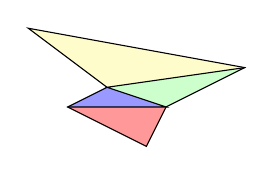
\begin{tikzpicture}[scale=1]

     
	
    % fill triangles
    \fill[red!40!white]   (0,0) -- ++(1,-0.5) -- ++(0.25,0.5) --cycle;
    \fill[blue!40!white]  (0,0) -- ++(1.25,0) --++(-0.75,0.25) --cycle;
    \fill[green!20!white]   (1.25,0) --++(-0.75,0.25) --++(1.75,0.25) --cycle;
    \fill[yellow!20!white]   (0.5,0.25) --++(1.75,0.25) --  ++(-2.75,0.5) --cycle;
	 
	% outline
	\draw (0,0) -- ++(1,-0.5) -- ++(0.25,0.5)-- ++(1,0.5) -- ++(-2.75,0.5)-- ++(1,-0.75)--cycle;

	% this is unrobust
	\draw (0,0) -- ++(1.25,0) --++(-0.75,0.25) --++(1.75,0.25);

\end{tikzpicture}
\caption{beispielhafte Triangluierung, $K_i$ disjunkt}
\label{AbbTriangulierung}
\end{center}
\end{figure}


\begin{figure}[h!]
\begin{center}
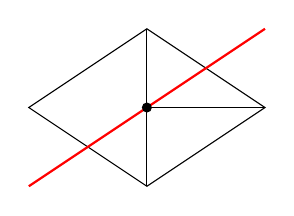
\begin{tikzpicture}[scale=1]

	% outline
	\draw (0,0) -- ++(1.5,-1) -- ++(1.5,1)-- ++(-1.5,1) -- cycle;
	\draw (1.5,-1) -- ++(0,2);
	\draw (1.5,0) -- ++(1.5,0);
	
	% red cross
	\draw[thick,red] (0,-1) --++ (3,2);

	% dot middle
	\filldraw (1.5,0) circle (1.6pt);

\end{tikzpicture}
\caption{Unzulässige Triangulierung}
\label{AbbUnzulaessigeTriangulierung}
\end{center}
\end{figure}
\end{enumerate}

\subsection*{Raum der stetigen stückweise linearen Funktionen}
\begin{align*}
V_h&:=\left\lbrace
\begin{array}{rl}
	v\in C(\overline{\Omega}) : &v|_{K_i}\in P_1(K)~\forall i=1,\ldots,N,\\
	&v|_{\partial\Omega}=0
\end{array}\right\rbrace
	\subseteq H^1_0(\Omega)\\
P_1(K_i)&=\spann(1,x,y)\\
P_2(K)&=\spann\big( x^\alpha, |\alpha|\leq k\big)\mit K\subseteq\R^d,~ x^{\alpha}:=x_1^{\alpha_1},\ldots,x_d^{\alpha_d}\\
Q_k(K)&=\spann\big(x^\alpha,\max\limits_i |\alpha_i|\leq k\big)\\
Q_1(K)&=\spann(1,x,y,xy)\\
\dim(V_h)&=\text{ Anzahl der inneren Knoten von der zulässigen Triangulierung}\\
\end{align*}

\begin{definition}[Finites Element]\enter %4.5
Ein \textbf{finites Element} ist ein Tripel $(K,V,\Sigma)$ mit:
\begin{enumerate}[label=(\roman*)]
\item $K\subseteq\R^d$ ist nichtleere offene, beschränkt und Lipschitz-berandet.
\item $V$ ist endlich-dimensionaler Funktionenraum von Funktionen mit Definitionsbereich $K$. $m:=\dim(V)$
\item $\Sigma$ ist eine Menge von $m$ linearen Funktionalen $\Sigma=\lbrace N_i\rbrace_{i\in\lbrace1,\ldots,m\rbrace}$, welche mindestend für alle Funktionen in $V$ definiert sind. Sie werden als \textbf{$V$-unisolvent} angenommen, d. h.:
\begin{align*}
\forall \alpha_1,\ldots\alpha_m:\exists! v\in V:\forall i\in\lbrace1,\ldots,m\rbrace:N_i(v)=\alpha_i
\end{align*}
Das bedeutet, es gibt Funktionen $v_i\in V$ mit
\begin{align*}
N_i(v_j)=\delta_{i,j}\qquad\forall i,j\in\lbrace1,\ldots m,\rbrace
\end{align*}
Die linearen Funktionale $N_i$ heißen \textbf{Nodal-Funktionen} oder \textbf{Freiheitsgrade (degrees of freedom / dof)}. die Funktionen $v_i$ sind die \textbf{lokale Basis} oder \textbf{Shape-Funktionen / Formfunktionen}.
\end{enumerate}
\end{definition}

\begin{definition}[affin äquivalente finite Elemente]\enter %4.6
Zwei finite Elemente $(K,V,\Sigma)$ und $(\hat{K},\hat{V},\hat{\Sigma})$ heißen \textbf{affin äquivalent}
\begin{align*}
:\Longleftrightarrow\exists F:\R^d\to\R^d\text{ affin \& invertierbar v.d.F. }
\hat{x}\mapsto B_k\cdot\hat{x}+b_k\mit B_k\in\R^{d\times d},b_k\in\R^d
\end{align*}
mit den Eigenschaften
\begin{enumerate}[label=(\arabic*)]
\item $\begin{aligned}
K=F(\hat{K})
\end{aligned}$
\item $\begin{aligned}
V=\Big\lbrace v: K\to\R:v=\hat{v}\circ F^{-1},\hat{v}\in\hat{V}\Big\rbrace
\end{aligned}$
\item $\begin{aligned}
\Sigma=\Big\lbrace N:V\to\R:N(v)=\hat{N}(v\circ F),~\hat{N}\in\hat{\Sigma}\Big\rbrace
\end{aligned}$
\end{enumerate}

\end{definition}

\begin{beisp}\

\begin{figure}[h!]
\begin{center}
\begin{figure}[h!]
	\center
	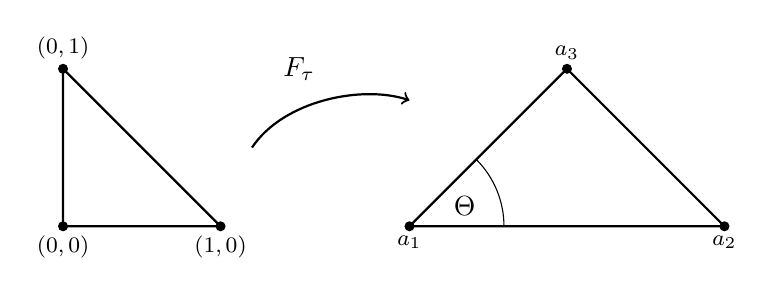
\begin{tikzpicture}[scale=2]

	
	


	% first simplix
	\draw[thick] (0,0) -- ++(0,1) -- ++(1,-1)--cycle;
	\filldraw (0,0)         circle (0.8pt);
	\filldraw (0,0) ++(1,0) circle (0.8pt);
	\filldraw (0,0) ++(0,1) circle (0.8pt);
	\fill[black,font=\footnotesize] (0,0) node[below] {$(0,0)$}
									(0,0) ++(1,0) node[below] {$(1,0)$}
									(0,0) ++(0,1) node[above] {$(0,1)$};
	
	%arrow
	\draw[thick,-to] (1.2,0.5) .. controls (1.4,0.8) and (1.9,0.9) .. (2.2, 0.8);
	
	%second simplex							
	\draw[thick] (2.2,0) -- ++(2,0) -- ++(-1,1)--cycle;
	\filldraw (2.2,0)         circle (0.8pt);
	\filldraw (2.2,0) ++(2,0) circle (0.8pt);
	\filldraw (2.2,0) ++(1,1) circle (0.8pt);
	\fill[black,font=\footnotesize] (2.2,0) node[below] {$a_1$}
									(2.2,0) ++(2,0) node[below] {$a_2$}
									(2.2,0) ++(1,1) node[above] {$a_3$};								
								
	
%	\pgfmathsetmacro{\ax}{2.2}
%	\pgfmathsetmacro{\ay}{0}
	
	\draw (2.2,0) ++(45:.6) arc (45:0:.6);
								
																		
	\node at (1.5,1) {$F_{\tau}$};
	\node at (2.55,0.13) {$\Theta$};				
	

	\end{tikzpicture}
		
	\caption{affine transformation}
	\label{ch1_plot_affin_equiv_triang}

\end{figure}
\caption{affin äquivalente Triangulierung}
\label{AbbAffinEquivTriang}
\end{center}
\end{figure}

\begin{align*}
F:\left\lbrace\begin{array}{l}
(0,0)\mapsto(a_1,a_2)\\
(1,0)\mapsto(b_1,b_2)\\
(0,1)\mapsto(c_1,c_2)
\end{array}\right.
\qquad\qquad
\begin{matrix}
\hat{N}_1(\hat{v})&=\hat{v}(0,0) &&N_1(v)=v(a_1,a_2)\\
\hat{N}_2(\hat{v})&=\hat{v}(1,0) &&N_2(v)=v(b_1,b_2)\\
\hat{N}_3(\hat{v})&=\hat{v}(0,1) &&N_3(v)=v(c_1,c_2)
\end{matrix}
\end{align*}
\end{beisp}

Sei $V$ ein Vektorraum mit Basis $\lbrace\varphi_1,\ldots,\varphi_m\rbrace$. Setze
\begin{align*}
\Sigma&=\lbrace N_1,\ldots,N_m\rbrace\\
M&=(m_{i,j}),\qquad m_{i,j}:=N_i(\varphi_j)\\
M&\text{ invertierbar }\Longleftrightarrow \text{ unisolvent}
\end{align*}
Unisolvenz: Gegeben $\alpha_1,\ldots\alpha_m\in\R$. Gibt es ein eindeutiges $v\in V$
\begin{align*}
N_i(v)&=\alpha_i,\qquad i\in\lbrace1,\ldots,m\rbrace\\
\stackrel{v=\sum\limits_{j=1}^m c_j\cdot\varphi_j}{\Longleftrightarrow}\quad
\sum\limits_{j=1}^m N_i(\varphi_j)\cdot c_j&=\alpha_i\\
\Longleftrightarrow
M\cdot c&=\alpha
\end{align*}

\begin{definition}[globales Nodal-Funktional / globale Freiheitsgrade (dof)]\enter
Seien $N_i^K$ und $N_j^{K'}$ zwei lokale Nodal-Funktionale von den finiten Elementen $(K,V,\Sigma)$ und $(K',V',\Sigma')$. Wir sagen, diese beiden lokalen Freiheitsgrade \textbf{gehören zum selben globalen Freiheitsgrad}
\begin{align*}
:\Longleftrightarrow N_i^K(\varphi|_K)=N_j^{K'}(\varphi|_{K'})\qquad\forall\varphi\in C^\infty(U)
\end{align*}
wobei $U$ eine offene Menge mit der Eigenschaft $\overline{K\cup K'}\subseteq U$ ist.\\
Die Menge aller globalen Freiheitsgrade bezeichnen wir mit $\Sigma_h$. Für $N\in\Sigma_h$ bezeichne $\Lambda(N)$ die Menge alle lokalen Freiheitsgrade, die zu $N$ gehören.
\end{definition}

\begin{definition}[Raum der finiten Elemente]\enter
Sei $\T_h$ eine Triangulierung von $\Omega$. Ein \textbf{Raum der finiten Elemente} $V_h$ ist gegeben durch 
\begin{align*}
V_h:=\left\lbrace v=(v_{K})_{K\in\T_h}\in\prod\limits_{K\in\mathcal{T}_h} V(K):N_i^K(v|_K)=N_j^{K'}(v|_{K'})~\forall N_i^K,N_j^{K'}\in\Lambda(N),\forall N\in\Sigma_h\right\rbrace
\end{align*}
wobei $(K,V(K),\Sigma(K)),K\in\T_h$ finite Elemente sind. Eine Funktion $v_h\in V_h$ ist eindeutig bestimmt durch die Werte von $N(v_h)$ von dem globalen Freiheitsgrad.
\end{definition}

Familie aller affin äquivlenten finiten Elementen
\begin{align*}
\big(K,V(K),\Sigma(K)\big)\sim\big(\hat{K},\hat{V},\hat{\Sigma}\big)
\end{align*}
Interpolation:
\begin{align*}
I_h(v):=\sum\limits_{i=1}^n N_i(v)\cdot\varphi_i\in V_h
\end{align*}
wobei $\Sigma_h=\lbrace N_1,\ldots,N_n\rbrace\text{ und }\lbrace\varphi_1,\ldots,\varphi_n\rbrace$ eine Basis von $V_h$ ist mit der Eigenschaft $N_i(\varphi_j)=\delta_{i,j}$.\\

\textbf{Wichtig: }
\begin{align*}
\big(I_h(v)\big)\big|_K&=I_h^K\big(v|_K\big)\quad\text{wobei}\\ I_h^K(v)&=\sum\limits_{i=1}^{m_K} N_i^{(K)}(v)\cdot\varphi_i^K,\qquad N_i^K(\varphi_j^K)=\delta_{i,j}\qquad\Sigma(K)=\left\lbrace N_1^K,\ldots,N_{m_K}^K\right\rbrace
\end{align*}

\begin{theorem}\label{theorem4.9}
Seien $K,\hat{K}\subseteq\R^d$ zwei affin äquivalente offene  Teilmengen des $\R^d$, d. h. es existiert eine affine bijektive Abbildung
\begin{align*}
F:\hat{K}\to K,\qquad \hat{x}\mapsto B_K\cdot\hat{x}+ b_K\qquad\mit B_K\in\R^{d\times d}\text{ invertierbar und }b_K\in\R^d
\end{align*}
Falls $v\in W^{m,p}(K)$ für $m\geq0,p\in[1,\infty)$, dann gehört $\hat{v}:=v\circ F$ zu $W^{m,p}(\hat{K})$ und wir erhalten
\begin{align*}
\big|\hat{v}\big|_{m,p,\hat{K}}\leq c\cdot\Vert B_K\Vert^m\cdot\big|\det(B_K)\big|^{-\frac{1}{p}}\cdot|v|_{m,p,K}
\end{align*}
wobei $c=c(m,d)$ eine Konstante ist und $\Vert\cdot\Vert$ eine Matrixnorm, die durch die euklidische Vektornorm induziert wird.\\
Zusätzlich gilt:
\begin{align*}
|v|_{m,p,K}&\leq c\cdot\Vert B_K^{-1}\Vert^m\cdot\big|\det(B_K)\big|^{\frac{1}{p}}\cdot|\hat{v}|_{m,p,\hat{K}}\\
F^{-1}(x)&=B_K^{-1}\cdot x-B_K^{-1}\cdot b_K
\end{align*}
\end{theorem}

\begin{lemma}\label{lemma4.10}
Seien $K,\hat{K}$ affin äquivalent mit $F(\hat{x})=B_K\cdot\hat{x}+b_K$. Dann gilt:
\begin{align*}
\Vert B_K\Vert&\leq\frac{h_K}{\hat{\rho}},\qquad\Vert B_K^{-1}\Vert\leq\frac{\hat{h}}{\rho_K}\qquad\text{wobei}\\
h_K&:=\diam(K):=\sup\limits_{x,y\in K}\Vert x-y\Vert\\
\rho_K&:=\sup\big\lbrace\diam(S):S\subseteq K\text{ Sphäre}\big\rbrace
\end{align*}
\end{lemma}
\begin{proof}
\begin{align*}
\Vert B_K\Vert&=\sup\limits_{z\neq0}\frac{\Vert B_K \cdot z\Vert}{\Vert z\Vert}=\frac{1}{\hat{\rho}}\cdot\sup\limits_{\Vert z\Vert=\hat{\rho}}\Vert B_K \cdot z\Vert
\end{align*}
Für alle $\eta$ mit $\Vert \eta\Vert=\hat{\rho}$ existieren zwei Punkte $\hat{x},\hat{y}\in\hat{K}$ so, dass $\eta=\hat{x}-\hat{y}$. Seien $x=F(\hat{x}),y=F(\hat{y})$. Dann gilt:
\begin{align*}
x-y&=B_K\cdot\hat{x}+b_K-\big(B_K\cdot\hat{y}+b_K\big)=B_K\cdot(\hat{x}-\hat{y})=B_K \cdot \eta\\
\Vert B_K\cdot \eta\Vert&=\Vert x-y\Vert\leq h_K\\
\implies \Vert h_K\Vert&\leq\frac{1}{\hat{\rho}}\cdot\sup\limits_{\Vert y\Vert=\hat{\rho}}\underbrace{\Vert B_K\cdot \eta\Vert}_{\leq h_K}\leq\frac{h_K}{\hat{\rho}}
\end{align*}
\end{proof}

\begin{lemma}[Deny-Lions]\label{lemma4.11DenyLions}\enter
Sei $P_r(K)$ der Raum aller Polynome mit höchstens Grad $r$. Dann gilt:
\begin{align*}
\exists c(K)>0:\inf\limits_{p\in P_r(K)}\Vert v+p\Vert_{r+1,p,k}\leq c(K)\cdot |v|_{r+1,p,k}\qquad\forall v\in W^{r+1,p}(K)
\end{align*}
\end{lemma}
\begin{proof}
\begin{align*}
n:=\dim \big(P_r(K)\big)=\begin{pmatrix}
r+d\\ d
\end{pmatrix}\text{ (Binomialkoeffizient)}
\end{align*}
Setze  für $\alpha\in\N_0^\alpha\mit|\alpha|\leq r $:
\begin{align*}
N_\alpha:W^{r+1,p}(K)\to\R,\qquad v\mapsto\int\limits_K D^\alpha v\d x\\
\alpha\longleftrightarrow x^\alpha =\prod\limits_{i=1}^d x_i^{\alpha_i}
\end{align*}
Also ist $\big\lbrace N_\alpha:|\alpha|\leq r\big\rbrace$ unisolvent auf $P_r(K)$.
\begin{align*}
\implies\left.
	\begin{array}{cl}
	N_\alpha(p)=0, &\falls\forall |\alpha|\leq r \\
	p\in P_r(K)&
	\end{array}
\right\rbrace
\implies p\equiv 0
\end{align*}
Wir werden die Ungleichung
\begin{align}\label{eqProof4.11Stern}\tag{$\ast$}
\Vert v\Vert_{r+1,p,K}\leq c(K)\cdot\left(|v|_{r+1,p,K}+\sum\limits_{|\alpha|\leq r}\big|N_\alpha (r)\big|\right)\qquad\forall v\in W^{r+1,p}(K)
\end{align}
indirekt zeigen. Angenommen, diese Ungleichung gilt nicht. Dann gibt es eine Folge $(v_l)_{n\in\N}$ mit 
\begin{align}
\Vert v_l\Vert_{r+1,p,K}=1\qquad\forall l\in\N\nonumber\\
\lim\limits_{l\to\infty} \left(|v|_{r+1,p,K}+\sum\limits_{|\alpha|\leq r}\big|N_\alpha (r)\big|\right)=0\label{eqProof4.11SternStern}\tag{$\ast\ast$}
\end{align}
Mit der kompakten Einbettung $W^{r+1,p}(K)\stackrel{c}{\hookrightarrow} W^{r,p}(K)$ erhalten wir:\\
Es gibt eine Teilfolge $(v_m)_{m\in\N}\subseteq(v_l)_{l\in\N}$, die in $W^{r,p}(K)$ gegen $v\in W^{r,p}(K)$ konvergiert.\\
Aus \eqref{eqProof4.11SternStern} folgt
\begin{align*}
\lim\limits_{m\to\infty}|v_m|_{r+1,p,K}=0\\
\end{align*}
Folglich ist $(v_m)_{m\in\N}$ eine Cauchyfolge in $W^{r+1,p}(K)$. Da $W^{r+1,p}(K)$ ein Banachraum ist, konvergiert diese Folge: $v_m\stackrel{m\to\infty}{\longrightarrow} v\in W^{r+1,p}(K)$ und somit $|v|_{r+1,p,K}=0$. Also $v\in P_r(K)$.
\begin{align*}
\left.\begin{array}{ll}
\stackrel{\eqref{eqProof4.11SternStern}}{\implies}
&N_\alpha(r)=0\qquad\forall |\alpha|\leq r\\
& v\in P_r(K)
\end{array}\right\rbrace\implies v=0
\end{align*}
Dies ist ein Widerspruch zu $\Vert v\Vert_{r+1,p,K}=1$. Also folgt \eqref{eqProof4.11Stern}.\\
Für jedes $v\in W^{r+1,p}(K)$ gibt es ein $q\in P_r(K)$ so, dass
\begin{align*}
N_\alpha(v)=-N_\alpha(q)\qquad\forall|\alpha|\leq n
\end{align*}
Es folgt
\begin{align*}
\inf\limits_{p\in P_r(K)}\Vert v+p\Vert_{r+1,p,K}
&\leq\Vert v+q\Vert_{r+1,p,K}\\
&\stackeq{\eqref{eqProof4.11Stern}}
c(K)\cdot\Big(\underbrace{|v+p|_{r+1,p,K}}_{=|v|_{r+1,p,K}}+\sum\limits_{|\alpha|\leq r}\underbrace{|N_\alpha(\cdot v+q)|}_{=0}\Big)
\end{align*}
\end{proof}

\begin{lemma}[Bramble-Hilbert]\label{lemma4.12BrambleHilbert}
Sei $(Y,\Vert\cdot\Vert_Y$ ein Banachraum und $F:W^{r+1,p}(K)\to Y$ linear mit den Eigenschaften
\begin{enumerate}[label=(\roman*)]
\item $\begin{aligned}
\big\Vert F(u)\Vert_Y\leq c_1\cdot\Vert u\Vert_{r+1,p,K}\qquad\forall u\in W^{r+1,p}(K)
\end{aligned}$ mit $c_1$ unabhängig von $u$.
\item $\begin{aligned}
F(p)=0\qquad\forall p\in P_r(K)
\end{aligned}$
\end{enumerate}
Dann gibt es Konstanten $c,\tilde{c}>0$ so, dass
\begin{align*}
\big\Vert F(u)\big\Vert_Y
\leq c\cdot\inf\limits_{p\in P_r(K)}\Vert u+p\Vert_{r+1,p,K}
\leq
\tilde{c}\cdot |u|_{r+1,p,K}\qquad\forall u\in W^{r+1,p}(K)
\end{align*}
\end{lemma}
\begin{proof}
\begin{align*}
F(u)&\stackeq{\text{Lin+(ii)}}F(u+p)\qquad\forall p\in P_r(K)\\
\big\Vert F(u)\big\Vert&=\inf\limits_{p\in P_r(K)}\Vert F(u+p)\big\Vert_Y\\
&\stackrel{\text{(i)}}{\leq}
c_1\cdot\inf\limits_{p\in P_r(K)}\Vert u+p\Vert_{r+1,p,K}\\
&\stackrel{\ref{lemma4.11DenyLions}}{\leq}
\tilde{c}\cdot |u|_{r+1,p,K}
\end{align*}
\end{proof}

\begin{lemma}\label{lemma4.13}
Seien $(\hat{K},\hat{V},\hat{\Sigma})$ und $(K,V,\Sigma)$ zwei affin-äquivalente Finite-Elemente wobei
\begin{align*}
F_k:\hat{K}\to K,\qquad\hat{x}\mapsto B_K\hat{x}+b_K
\end{align*}
Dann gilt:
\begin{align*}
(I_K v)\circ F_k=\hat{I}(v\circ F_K)
\end{align*}
wobei $\hat{I}_K$ und $I_K$ die Interpolations-Operatoren auf $\hat{K}$ bzw. $K$.
\end{lemma}
\begin{proof}
\begin{align*}
\hat{I}\hat{v}&=\sum\limits_{i=1}^m\hat{N}_i(\hat{v})\cdot\hat{\varphi}_i\\
I_K v&=\sum\limits_{i=1}^m N_i(v)\cdot\varphi,\qquad \varphi_i\circ F_K=\hat{\varphi},\qquad N(v)=\hat{N}(v\circ F_K)
\end{align*}
\end{proof}

\begin{theorem}\label{theorem4.14}
Sei
\begin{itemize}
\item $(\hat{K},\hat{V},\hat{Sigma})$ Finites-Element
\item $m,r\in\N_0$
\item $p,q\in[1,\infty]$
\end{itemize}
so, dass
\begin{enumerate}[label=(\roman*)]
\item $\begin{aligned}
E^{r+1,p}(\hat{K})\hookrightarrow W^{m,q}(\hat{K})
\end{aligned}$
\item $\begin{aligned}
p_r(\hat{K})\subseteq\hat{V}\subseteq W^{m,q}(\hat{K})
\end{aligned}$
\item $\begin{aligned}
\hat{N}_i
\end{aligned}$ lineare stetige Funktionale auf
\begin{align*}
W^{r+1,p}(\hat{K})\qquad\forall\hat{N}_i\in\hat{\Sigma}
\end{align*}
\end{enumerate}
Dann existiert eine Konstante $c(\hat{K},\hat{V},\hat{\Sigma})$ so, dass
\begin{align*}
\big| v-I_K v\big|_{m,q,K}\leq c(\hat{K},\hat{V},\hat{\Sigma})\cdot\big(\meas(K)\big)^{\frac{1}{q}-\frac{1}{p}}\cdot\frac{h_K^{r+1}}{\rho_K^m}|v|_{r+1,p,K}
\end{align*}
für alle $v\in E^{r+1,p}(K)$ wobei $(K,V,\Sigma	)$ ist affin-äquivalent zu $(\hat{K},\hat{V},\hat{\Sigma})$ und
\begin{itemize}
\item $\meas(K)$ ist das $d$-dimensionale Maß von $K$
\item $h_K:=\diam(K)$
\item $\rho_K$ ist der Diameter der größten Kugel in $K$
\end{itemize}
Im Fall $p=q=2,m=1,\rho_K\sim h_K$ erhält man
\begin{align*}
\big|v-I_K v\big|_{1,2,K}\leq \hat{c}\cdot h_K^r\cdot |v|_{r+1,2,K}
\end{align*}
\end{theorem}
\begin{proof}
\begin{align*}
\big\Vert \hat{I} \hat{v} \big\Vert_{m,q,\hat{K}} \\
&=\left\Vert \sum\limits_{i=1}^m \hat{N}_i(\hat{v}) \cdot \hat{\varphi}_i \right\Vert_{m,q,K} \\
&\leq \sum\limits_{i=1}^m \big| \hat{N}_i(\hat{v}) \big| \cdot \big\Vert \hat{\varphi}_i \big\Vert_{m,q,\hat{K}} \\
&\leq \underbrace{\left( \sum\limits_{i=1}^m c\cdot \big\Vert \hat{\varphi}_i \big\Vert_{m,q,\hat{K}}\right)}_{=:c(\hat{K},\hat{V},\hat{\Sigma})}\cdot\Vert\hat{v}\Vert_{r+1,p,\hat{K}} \\
&\implies \hat{I}:W^{r+1,p}(\hat{K})\to W^{m,q}(\hat{K})\text{ist stetig}
\end{align*}
Auf $P_r(\hat{K})\subseteq V$ folgt $\hat{I}\hat{p}=\hat{p}$ für alle $\hat{p}\in P_r(\hat{K})$. Es folgt
\begin{align*}
\hat{v}-\hat{I}\hat{v}
&=\big(\hat{v}+\hat{p}\big)-\hat{I}\big(\hat{v}+\hat{p}\big) \\
&=\big(\id -\hat{I}\big)\big(\hat{v}+\hat{p}\big) 
\qquad\forall \hat{v}\in W^{r+1,p}(\hat{K}),\forall \hat{p}\in P_r(\hat{K})\\
\end{align*}
\begin{align*}
\big| \hat{v}-\hat{I} \hat{v} \big|_{m,q,\hat{K}}
&=\Big| \big( \id - \hat{I} \big) \big( \hat{v}+\hat{p} \big) \Big|_{m,q,\hat{K}} \qquad\forall\hat{p}\in P_r(\hat{K})\\
&\leq \inf\limits_{\hat{p}\in P_r(\hat{K})} \Big| \big(\id-\hat{I}\big) \big(\hat{v}+\hat{p}\big) \Big|_{m,q,\hat{K}}\\
&\leq c(\hat{K},\hat{V},\hat{\Sigma})\cdot\inf\limits_{\hat{p}\in P_r(\hat{K})}\big\Vert\hat{v}+\hat{p}\big\Vert_{r+1,p,\hat{K}} \\
&\stackrel{\ref{lemma4.11DenyLions}}{\leq}
c(\hat{K},\hat{V},\hat{\Sigma})\cdot\big|\hat{v}\big|_{r+1,p,\hat{K}}
\end{align*}
Aus dem vorherigen Lemma \ref{lemma4.13} folgt:
\begin{align*}
&\big(v-I_K J v\big)\circ F_K=\underbrace{v\circ f_K}_{=:\hat{v}}-\hat{I}(v\circ F_K)=\hat{v}-\hat{I}\hat{v}\\
\big| v-I_K v\big|_{m,q,K} \\
&\stackrel{\ref{theorem4.9}}{\leq}
c\cdot\big\Vert B_K^{-1}\big\Vert^m\cdot\big|\det(B_K)\big|^{\frac{1}{q}}\cdot\big|\underbrace{(v-I_K v)\circ F_K}_{=\hat{v}-\hat{I}\hat{v}}\big|_{m,q,K}\\
&\leq c\cdot\big\Vert B_K^{-1}\big\Vert\cdot|\det(B_K)|^{\frac{1}{p}}\cdot\big|\hat{v}\big|_{r+1,q,\hat{K}}\\
&\stackrel{\ref{theorem4.9}}{\leq}
c\cdot\big\Vert B_K^{-1}\big\Vert^m\cdot\Vert B_K\Vert^{r+1}\cdot|\det(B_K)|^{\frac{1}{q}-\frac{1}{p}}\cdot |v|_{r+1,p,K}\\
&\stackrel{\ref{lemma4.10}}{\leq}
c\cdot\frac{\hat{h}^m}{\hat{\rho}^{r+1}}\cdot\frac{h_K^{r+1}}{\rho^m}\cdot|\det(B_K)|^{\frac{1}{q}-\frac{1}{p}}\cdot|v|_{r+1,q,K}\\
\meas(K)&=\int\limits_K 1\d x=\int\limits_{\hat{K}}\big|\det(B_K)\big|\d\hat{x}=\big|\det(B_K)\big|\cdot\underbrace{\meas(\hat{K})}_{\longrightarrow c(\hat{K},\hat{V},\hat{\Sigma})}\\
&\implies
\big| v-I_K v\big|_{m,q,K}
\leq c\cdot\frac{h_K^{r+1}}{\rho_K^m}\cdot\big|\meas(K)\big|^{\frac{1}{q}-\frac{1}{p}}\cdot|v|_{r+1,p,K}
\end{align*} 
\end{proof}





